\ProvidesFile{thesis.tex}[2025-01-15 PurdueThesis thesis.tex file]

%  The home page for the PurdueThesis software is
%      https://engineering.purdue.edu/~mark/PurdueThesis/
%
%  Be sure to sign up for the PurdueThesis mailing list at
%      https://engineering.purdue.edu/ECN/mailman/listinfo/purduethesis-list
%  so you learn of new versions of this software.  You must be on that
%  mailing list to receive help with this software.
%
%  This is the template root file for an example thesis (for master's
%  degree) or dissertation (for a Ph.D.).  From now on "thesis" will
%  refer to both of these unless stated otherwise.
%
%  LaTeX systems include auxiliary programs to do bibliographies,
%  indexes, etc.  The latexmk program runs the fewest programs needed
%  to update your thesis.
%
%  On Overleaf (run LaTeX on the web) clicking 'Recompile' will recompile
%  your thesis.
%
%  Use this command on Linux to do all the steps needed to compile your thesis.
%    For Mark Senn:
%      Use
%          latexmk -e '$biber="biber --output-safechars"' -f -g -lualatex --shell-escape thesis
%      to get extra debugging information printed.  Sometimes the `-f -g' can 
%      be deleted to run faster.
%    For everyone else:
%      Use
%          latexmk -e '$biber="biber --output-safechars"' -f -g -lualatex thesis
%      Sometimes the `-f -g' can be deleted to run faster.
%  Here is how that command works:
%      latexmk
%          The latexmk program figures out how to compile
%          your thesis in the quickest way.
%      -e '$biber="biber --output-safechars"'
%          Add the '--output-safechars' option to biber,
%          the command that makes your references.  This
%          command makes accented characters in your references
%          work ok.
%      -f
%          Force latexmk to process your entire thesis, even
%          if it contains errors.
%      -g
%          Force latexmk to process document fully, even under situations
%          where latexmk would normally decide that no changes in the
%          source files have occurred since the previous run.  This  option
%          is  useful, for example, if you change some options and wish to
%          reprocess the files.
%      -lualatex
%          The -lualatex option process your thesis using the LuaLaTeX
%          version of LaTeX.  LuaLaTeX has the Lua programmng language
%          added to make programming LaTeX easier.  You won't need to
%          learn Lua or do any LaTeX programming for your thesis.
%      --shell-escape
%          The --shell-escape option allows you to run external programs
%          from inside your thesis.
%      thesis
%          Process your thesis.tex file.
%
%
%  NOTE TO SELF
%      To count the number of references see
%          https://tex.stackexchange.com/questions/66829/count-number-of-references-using-biblate
%      See set the \labelnumberwidth see page 316 of
%          https://ctan.math.illinois.edu/macros/latex/contrib/biblatex/doc/biblatex.pdf
%      
%
%  PROGRAM                                       BIBLIOGRAPHY    PurdueThesis.cls    thesis.tex   WORKS
%                                                STYLE           RCS rev             RCS rev
%  Mathematics                                   apa             1.249               1.58         yes
%  Mathematics                                   ieee            1.250               1.59         yes
%  Electrical and Computer Engineering           ieee            1.250               1.60         yes
%  Earth, Atmospheric, and Planetary Sciences    apa             1.251               1.61         yes
%  Mathematics                                   apa             1.252               1.62         yes
%  Technology Leadership and Innovation          apa             1.253               1.63         yes
%  Mathematics                                   numeric         ????                ????         ????
%  Earth, Atmospheric, and Planetary Sciences    apa             ????                ????         ????
%

%
%  References cited below:
%
%  TM2017 is short for Thesis Manual 2017:
%    A Manual for the Preparation of Graduate Theses,
%    eighth revised edition,
%    Thesis and Dissertation Office,
%    Purdue University,
%    2017,
%    revised August 30, 2017,
%    http://www.purdue.edu/gradschool/documents/thesis/graduate-thesis-manual.pdf,
%    last retrieved on May, 8, 2021.
%
%  In this file, change the example information to your information.
%


% author
% Put your name here.
\newcommand{\ZZauthor}{Timothy J. Wiegman}


% campus
% Choose a campus from the following list:
%     VALUE               COMMENT
%     Bloomington
%     Fort Wayne
%     Hammond
%     Indianapolis
%     Manoa               don't include the macron character here,
%                         it will get printed automatically
%     Reno
%     Westville
%     West Lafayette
\newcommand{\ZZcampus}{West Lafayette}
% \newcommand{\ZZcampus}{Fort Wayne}


% degree
% If you are in `Motorsports Engineering'
% use `Master of Science in Mechanical Engineering'.
% Choose a degree from the following list:
%     Doctor of Audiology
%     Doctor of Nursing Practice
%     Doctor of Philosophy
%     Doctor of Technology
%     Master of Arts
%     Master of Fine Arts
%     Master of Library Science
%     Master of Science
%     Master of Science in Agriculture
%     Master of Science in Aviation and Aerospace Management
%     Master of Science in Aeronautics and Astronautics
%     Master of Science in Agricultural and Biological Engineering
%     Master of Science in Building Construction Management
%     Master of Science in Biomedical Engineering
%     Master of Science in Chemical Engineering
%     Master of Science in Civil Engineering
%     Master of Science in Education
%     Master of Science in Electrical and Computer Engineering
%     Master of Science in Engineering
%     Master of Science in Engineering Technology
%     Master of Science in Human Resources Management
%     Master of Science in Industrial Engineering
%     Master of Science in Industrial Technology
%     Master of Science in Mechanical Engineering
%     Master of Science in Materials Engineering
%     Master of Science in Nuclear Engineering
\newcommand{\ZZdegree}{Master of Science in Agricultural and Biological Engineering}
% \newcommand{\ZZdegree}{Master of Science}


% document
% Choose a document from the following list:
%     A Dissertation
%     A Master's Bypass Report
%     A Preliminary Report
%     A Thesis
% \newcommand{\ZZdocument}{A Dissertation}
\newcommand{\ZZdocument}{A Thesis}

% graduation
% Chose a month from
%     May
%     August
%     December
% followed by a space
% then choose a year from 2020 to 2030.
\newcommand{\ZZgraduation}{May 2025}


% institution
% Choose an institution name from the following list:
%     VALUE                   COMMENT
%     Purdue University
%     University of Hawaii    don't include the 'okina character here,
%                             it will get printed automatically
\newcommand{\ZZinstitution}{Purdue University}


% program
% Choose a program from the following list:
% If you are in `Motorsports Engineering' use `Mechanical Engineering'.
%     VALUE
%     Aeronautics and Astronautics
%     Agricultural and Biological Engineering
%     Agricultural Economics
%     Agronomy
%     American Studies
%     Animal Sciences
%     Anthropology
%     Applied Physics
%     Art and Design
%     Aviation and Transportation Technology
%     Basic Medical Sciences
%     Biochemistry
%     Biological Sciences
%     Biology
%     Biomedical Engineering
%     Botany and Plant Pathology
%     Chemical Engineering
%     Chemistry
%     Chemistry and Chemical Biology
%     Child Development and Family Studies
%     Civil and Construction Engineering
%     Civil and Mechanical Engineering
%     Communication
%     Communications
%     Comparitive Pathobiology
%     Computer and Information Science
%     Computer and Information Technology
%     Computer Graphics Technology
%     Computer Science
%     Construction Management Technology
%     Consumer Science
%     Curriculum and Instruction
%     Earth, Atmospheric, and Planetary Sciences
%     Economics
%     Educational Studies
%     Electrical and Computer Engineering
%     Engineering Education
%     Engineering Technology
%     English
%     Entomology
%     Food Science
%     Forensic and Investigative Sciences
%     Forestry and Natural Resources
%     Health and Kinesiology
%     Health Sciences
%     History
%     History and Philosophy
%     Horticulture
%     Hospitality and Tourism Management
%     Human Development and Family Studies
%     Industrial and Physical Pharmacy
%     Industrial Engineering
%     Interdisciplinary Biomedical Studies Program
%     Interdisciplinary Studies (Comparitive Literature)
%     Languages and Cultures
%     Linguistics
%     Management
%     Materials Engineering
%     Mathematical Sciences
%     Mathematics
%     Mechanical and Energy Engineering
%     Mechanical Engineering
%     Mechnical and Civil Engineering
%     Medicinal Chemistry and Molecular Pharmacology
%     Nuclear Engineering
%     Nursing
%     Nutrition Science
%     Organizational Behavior and Human Resource Management
%     Pharmacy Practice
%     Philosophy
%     Philosophy and Literature
%     Physics
%     Physics and Astronomy
%     Political Science
%     Psychological Sciences
%     Sociology
%     Speech, Language, and Hearing Sciences
%     Statistics
%     Technology
%     Technology Leadership and Innovation
%     Theatre
%     Veterinary Clinical Sciences
%     Youth Development and Agricultural Education
\newcommand{\ZZprogram}{Agricultural and Biological Engineering}
% \newcommand{\ZZprogram}{Applied Physics}


% title
% If you need to manually split the title,
% over several lines do, for example,
%     \newcommand{\ZZtitle}{%
%       This is the First Line\\[-6pt]
%       and this is the Second Line%
%     }
\newcommand{\ZZtitle}{Computer Vision Analysis \& Monitoring of Vegetation Control
Operations on Indiana Roadsides}


% showcolophon
% Print the ap-colophon.tex file at the end of the document?
% THE SUBMITTED COPY OF YOUR THESIS MUST BE RUN WITH ZZshowcolophon SET TO false.
\newcommand{\ZZshowcolophon}{false}

% showdiagonalline
% Show a diagonal line from lower left to center
% of main printed part of page?
% THE SUBMITTED COPY OF YOUR THESIS MUST BE RUN WITH ZZshowdiagonalline SET TO false.
\newcommand{\ZZshowdiagonalline}{false}

% showgridlines
% Show grid lines on main printed part of page
% Vertical and horizontal grid lines are put
% in the normal printed part of the page---this
% includes lines where the margins are.
% THE SUBMITTED COPY OF YOUR THESIS MUST BE RUN WITH ZZshowgridlines SET TO false.
\newcommand{\ZZshowgridlines}{false}

% showmarginlines
% Show margin lines on the edge of the normal printed part of the page?
% Margin lines show where the margins are.
% THE SUBMITTED COPY OF YOUR THESIS MUST BE RUN WITH ZZshowmarginlines SET TO false.
%     VALUE    MEANING
%     false    don't show marginlines
%     true     show marginlines
\newcommand{\ZZshowmarginlines}{false}

% showtimestamp
% Show, for example, a "compiled on  2021-03-02  Tuesday  17:16:24"
% timestamp in the upper right corner of page?
%     VALUE    MEANING
%     false    don't show timestamp
%     true     show timestamp
% THE SUBMITTED COPY OF YOUR THESIS MUST BE RUN WITH ZZshowtimestamp SET TO false.
\newcommand{\ZZshowtimestamp}{false}

% showtodonotes
% Set things up for todonotes.
%     VALUE    MEANING
%     false    don't put todo notes in PDF file
%     true     put 0.8 inch wide todo notes in PDF file
%     wide     put 3.8 inch wide todo notes in PDF file, do not send
%              todonotes = wide output to a printer
% THE SUBMITTED COPY OF YOUR THESIS MUST BE RUN WITH ZZshowtodonotes SET TO false.
\newcommand{\ZZshowtodonotes}{false}

% Mark Senn uses an "optional-debugging-code.tex file" but does not
% distribute it.  The following line won't do anything if you don't
% have an optional-debugging-code.tex file so you can leave it the
% way it is.
\InputIfFileExists{optional-debugging-code.tex}{}{}

% The \includeonly command can be used to only include some
% files that have \include commands below.  This is handy
% to only include some files so your document will LaTeX
% faster or if you're trying to narrow down where an error
% occurs.  You can use
%   \includeonly{ch-introduction}
% to only include ch-introduction.tex, or
%   \includeonly{ch-introduction,ap-about-appendices}
% to include ch-introduction.tex and ap-about-appendices.tex.
% More files can be added---just put ',' between the names.
% Comment out the following line before submitting the
% final copy of your thesis.
%\includeonly{ch-introduction,ap-about-appendices}


\documentclass{PurdueThesis}

% I'm not using the silence package to not print LaTeX errors
% and warnings because
%     \usepackage{silence}
% caused
%     [89] [90] [91] (./z.out) (./z.out^C 
%     ! Interruption.
%     \sl@StoreMessage ...oveGobbletwo #1\sl@Terminator 
%                                                       \@gobbletwo \sl@Terminator...
%     
%     l.2 \subsection{Sum of 1 to \(n\) example}
%                                             
%     ? 
% where ^C indicates I typed a Control-C because LaTeX was 'stuck'.
%
% I do the following when using Overleaf.  Check the icon just to the
% right of the 'Recompile' button to see how many errors/warnings there
% are.  If that number goes up I look for the details of what has
% changed.
% \usepackage{silence}

%%%% \ExplSyntaxOn                         %%%% changed 2021-07-27 by mark
%%%% \bool_set_true:N \ZZCenterCaptionB    %%%% changed 2021-07-27 by mark
%%%% \ExplSyntaxOff                        %%%% changed 2021-07-27 by mark

\newcommand{\ZZatinformation}{}
% If you are at the Hammond or Westville campus
% remove the "%" from the begining of the next line.
%\newcommand\ZZatinformation{~at~Purdue~Northwest}


% PurdueThesis.cls loads the rotating package which loads the graphicx
% package.  From page 12 of "Packages in the `graphics' bundle", 2021-03-05,
% retrieved 2021-06-16, at https://texdoc.org/serve/grfguide.pdf/0
%     \graphicspath{<dir-list>}
%
%         This optional declaration may be used to specify a list of
%         directories in which to search for graphics files.  The
%         format is the same as for the LaTeX 2e primitive \input@path.
%         A list of directories, each in a {} group (even if there is
%         only one in the list).  For example:
%             \graphicspath{{eps/}{tiff/}}
%         would cause the system to look in the subdirectories eps and
%         tiff of the current directory.  (All modern TeX systems use /
%         as the directory separator, even on Windows.)
%
%         The default setting of this path is \input@path that is:
%         graphics files will be found whereever TeX files are found.
%
% Look in the "graphics" subfolder for graphics files.
% This is done to reduce the number of files in the main thesis folder
% so the ones in there are easier to find.
\graphicspath{{graphics/}}

% Look in the `misc' subfolder for miscellaneous files
% PurdueThesis.cls and thesis.tex need.  Look in the `packages'
% subfolder for packages.  This is done to reduce the number of files
% in the main thesis folder so the ones in there are easier to find.
%%%%\ExplSyntaxOn
%%%%  \seq_set_from_clist:Nn \l_file_search_path_seq {misc,packages}
%%%%\ExplSyntaxOff
\makeatletter
  \def\input@path{{misc}{packages}}
\makeatother

% The BibLaTeX bibstyle and citestyle are chosen automatically based
% on your program (e.g., `Mathematics').  For example, if you are in
% the Mathematics program normally you are using the `numeric'
% bibstyle and citestyle.
% the `numeric-comp' (numeric compressed---instead of '[1,2,3]' use
% '[1--3]') citestyle.
% To override the bibstyle and citestyle to `apa' use
%     \ZZoverridebibstyle{apa}
% To override the bibstyle to `apa'and the citestyle to `numeric-comp'
% use
%     \ZZoverridebibstyle{apa}
%     \ZZoverridecitestyle{numeric-comp}
% Any overrides must go before the \ConfigureBibliography.
%%%\ZZoverridebibstyle{apa}

\ConfigureBibliography

% \DeclareSourcemap
%   {
%     \maps[datatype=bibtex]
%     {
%       % Ignore "urldate = {...}" in .bib files.
%       % See the first complete example on page 201 of
%       %     https://mirrors.rit.edu/CTAN/macros/latex/contrib/biblatex/doc/biblatex.pdf
%       \map
%         {
%           \step[fieldset=urldate, null]
%         }
%       % Enter approximate (circa) dates using, for example,
%       % "year = c2020"  See
%       %     https://tex.stackexchange.com/questions/224617/what-is-the-correct-way-to-handle-approximate-dates-in-biblatex
%       \map[overwrite=false]
%         {
%           \step[fieldsource=year]
%           \step[fieldset=sortyear, origfieldval, final]
%           \step[fieldsource=sortyear, match={c}, replace={}]
%         }
%     }
%   }

% For \bm.
% The bm package was last updated on 2022-01-05.
\usepackage{bm}

% To let {\bfseries\scshape text} work as expected.
% See
%     https://tex.stackexchange.com/questions/27411/small-caps-and-bold-face
\usepackage{bold-extra}

% For chemical figures.
\usepackage{chemfig}

% For typesetting cryptography pseudocode, algorithms, and protocols.
% See
%     https://mirror.las.iastate.edu/tex-archive/macros/latex/contrib/cryptocode/cryptocode.pdf
\usepackage
[
  n,            % or lambda
  advantage,
  operators,
  sets,
  adversary,
  landau,
  probability,
  notions,
  logic,
  ff,
  mm,
  primitives,
  events,
  complexity,
  oracles,
  asymptotics,
  keys,
]
{cryptocode}

% Define
%    \VerbatimInput[options]{filename}
%    \begin{VerbatimOut}{filename} ... \end{VerbatimOut}.
\usepackage{fancyvrb}
  % So '|verbatim|' will print 'verbatim' in a typewriter font.
  % If you don't want this, put a '%' before the next line.
  \DefineShortVerb{\|}

% For \InpuutIfFileExists.
\usepackage{filehook}

% Use OpenType fonts in LuaLaTeX.
\usepackage{fontspec}

% For nlui testing.
\usepackage{listings}

% For chemical equations.
% See
%     https://ctan.org/pkg/mhchem?lang=en
% From the "Package documentation" linked-to document
%     mhchem needs a couple of other packages.
%     For instance, expl3, amsmath and calc.
\usepackage[version=4]{mhchem}
  % If I'm loading the package to just define a few new commands I'll indent
  % two spaces right after loading the package and define the few new
  % commands here.  If I'm defining more than a few commands I usually do it
  % after loading all the packages.
  % Define "\nitrate" to be the chemical symbol for nitrate.
  \newcommand{\nitrate}{\ce{NO3{-}}}
  % Define "\pnitrate" (short for "parenthesized nitrate") to be the chemical
  % symbol for nitrate surrounded by parentheses.
  \newcommand{\pnitrate}{(\nitrate)}
  % "Define \vpnitrate" (short for "verbose parenthesized nitrate") to be
  % the word "nitrate" followed by a space followed by the chemical symbol
  % for nitrate with parentheses around it.
  \newcommand{\vpnitrate}{nitrate (\nitrate)}

% For
%     \cancel
%     \highlight
% See
%     http://ftp.math.purdue.edu/mirrors/ctan.org/macros/latex/contrib/siunitx/siunitx.pdf
% pages 11--12.
\usepackage{cancel}


% Redefine description, enumerate, and itemize lists.
% See
%     https://mirrors.concertpass.com/tex-archive/macros/latex/contrib/enumitem/enumitem.pdf
% \usepackage{enumitem}
% \setlist[itemize]{leftmargin=7pt,rightmargin=24pt}



% This gets rid of
%     [5] (./thesis.toc
%     ! Undefined control sequence.
%     \vbox_set:Nn ...box:D {\color_group_begin: #2\par
%                                                       \color_group_end: }
%     l.32 ...}Basic Circuit Components}{31}{section.67}
%                                                       %
%     ?
% and
%     [6]
%     ! Undefined control sequence.
%     \vbox_set:Nn ...box:D {\color_group_begin: #2\par
%                                                       \color_group_end: }
%     l.61 ...rline {P.1}Frenchspacing}{67}{section.445}
%                                                       %
%     ?
% errors.
% See
%     https://github.com/latex3/latex2e/issues/73
\usepackage{etoc}

% Define \setmaxprintline{number_of_columns}.
% \usepackage{hardwrap}

% Include XMP data in a PDF document.
% See
%   http://mirrors.ibiblio.org/CTAN/macros/latex/contrib/hyperxmp/hyperxmp.pdf
% for more information including all the possible fields that can be set.
\usepackage{hyperxmp}
  \hypersetup{
    pdfauthor    = {Timothy J Wiegman},
    pdfcopyright = {Copyright \copyright\ 2025 by Timothy Wiegman.  All rights reserved.},
    % Use `yyyy-mm' format where `yyyy' is year and `mm' is month.
    pdfdate      = {2025-05},
    pdfkeywords  = {LaTeX; Purdue University; PurdueThesis},
    pdflang      = {en},
    pdfpublisher = {Purdue University},
    pdfsubject   = {%
                     PurdueThesis is a LaTeX document class used for
                     master's bypass reports,
                     master's theses,
                     PhD dissertations,
                     and PhD preliminary reports.
                     This template demonstrates how to use PurdueThesis.%
                   },
    pdftitle     = {Wiegman-MSABE-Thesis},
  }


% For `\Box'.
\usepackage{latexsym}

% Used in ap-colophon.tex.
\usepackage{luacode}

% For indexing.  Making an index is optional.
% Make these commands available:
%     COMMAND           DESCRIPTION
%     \index{string}    put "string" in index information
%     \makeindex        save information to make the index
%     \printindex       print the index
% See
%     https://ctan.org/pkg/makeidx?lang=en
% for more information.
\usepackage{makeidx}
  % By default \index ignores its argument.
  % This activates indexing.
  \makeindex
  % The "chapter name" for the index.
  \renewcommand{\indexname}{INDEX}

% The mathtools package
% (see http://mirror.utexas.edu/ctan/macros/latex/required/amsmath/amsmath.pdf)
% loads the amsmath package which defines the
%     align
%     align*
%     alignat
%     alignat*
%     equation
%     equation*
%     flalign
%     flalign*
%     gather
%     gather*
%     multitaper
%     multitaper*
%     split
% environments and extends amsmath by defining many other commands.
% See
%     https://ctan.org/pkg/amsmath
% for information about amsmath and
%     http://ctan.math.washington.edu/tex-archive/macros/latex/contrib/mathtools/mathtools.pdf
% for information about mathtools.
\usepackage{mathtools}

% Define \includemedia.
\usepackage{media9}

% Define \begin{multicols}{number_of_columns} ... \end{multicolumns}.
% Used in ap-text.tex.
\usepackage{multicol}

% Define \ditto.
\usepackage{pa-ditto}

% Define \FigureDash.
% \FigureDash is a dash the width of a digit in the current font.
\usepackage{pa-figure-dash}

% For PurdueThesis, PuTh, TeX, LaTeX, METAFONT, METAPOST, ... logos.
\usepackage{pa-logos}

\usepackage{pdfpages}

% Follow ISO 80000-2:2019:
%   o  The e, i, j, and pi constants should be in an upright font.
%   o  The ordinary derivative operator d should be in an upright font.
\usepackage{pa-mismath}
  % For letter in ('e', 'i', 'j'):
  %     o  \MathUp{letter} typesets letter in an upright font from now on.
  %        Use \mathit{letter} to get a math italic letter
  %        when Mathup{letter} is active.
  %     o  \MathIt{letter} typesets letter in a math italic font from now on.
  %        Use \mathup{letter} to get an upright letter
  %        when MathIt{letter} is active.
  %
  % \pinumber typesets pi in an upright font from now on.
  %  Use \itpi to get a math italic pi when \pinumber is active.
  %  
  % \pinormal typesets pi in a math italic font from now on.
  % Use \text{\pi} to get an upright pi when \pinormal is active.
  %
  % Adjust these are needed for your document.
  \MathUp{e}  \MathUp{i}  \MathUp{j}  \pinumber
  %
  % Use \di for ordinary derivative operator.
  
% This does not depend on the pa-mismath package.
% Do more ISO 80000-2:2019 stuff.
% Follow ISO 80000-2:2019:
%   o  The partial derivative operator should be in an upright font.
% The pa-mismath package defines "\di" as the ordinary differential operator.
% Define "\pa" as the partial derivative operator.
\def\pa{\rotatebox[origin=c]{14}{\partial}}

% This does not depend on the pa-mismath package.
% Do more ISO 80000-2:2019 stuff.
% Follow ISO 80000-2:2019:
%   o  Use \mathcal{F} for the Fourier transform.
\def\Fourier{\mathcal{F}}

% This does not depend on the pa-mismath package.
% Do more ISO 80000-2:2019 stuff.
% Follow ISO 80000-2:2019:
%   o  Use \mathcal{L} for the Laplace transform.
\def\Laplace{\mathcal{L}}

% Define \MyRepeat{what}{repeat}.
% Do "what" "repeat" number of times.
\usepackage{pa-repeat}

% Define \FloatBarrier.
% \FloatBarrier process all unproccesed floats (tables, figures, etc.).
\usepackage{placeins}

% Define \hl.
% Undefine \st so soul will load without an error.
% I hope \st wasn't used for something important!
\let\st\relax
\usepackage{soul}

% Define \textcent.
\usepackage{textcomp}

% !!! This doesn't work yet, figure it out later.
% For \textprimstress.
% \usepackage{tipa}

% Needed for chapter "Graphics", section "TikZ and PGF".
\usepackage{tikz}
  % Needed to customize arrows.
  \usetikzlibrary{arrows.meta}
  % For electrical diagrams.
  % Uses the TikZ package.
  % The circuitikz name is short for "circuit TikZ".
  \usepackage{circuitikz}
  %
  \usepackage{menukeys}
  %
  % Needed for 3D TikZ stuff.
  \usetikzlibrary{3d}
  %
  % Needed for pa-typographic-conventions package.
  \usetikzlibrary{calc,shadows,shapes.misc,shapes.symbols}
  %
  % Needed for putting text along a path.
  \usetikzlibrary{decorations.text}
  %
  % Draw TikZ decorations.
  % Needed for at least the Kalman filter system model graphic.
  \usetikzlibrary{decorations.pathmorphing} % noisy shapes
  %
  % Fit shapes to coordinates.
  % Needed for at least the Kalman filter system model graphic.
  \usetikzlibrary{fit}
  %
  % Draw the background after the foreground.
  \usetikzlibrary{backgrounds}	% drawing the background after the foreground

% Needed for the Feynman diagram in ap-physics.tex.  Tikz-feynman
% requires LuaLaTeX instead of pdflatex be run.  LuaLaTeX screws up
% the horizontal position of the list of figures---this is a known bug.
% The Thesis Office accepts theses with this problem.
\usepackage[compat=1.1.0]{tikz-feynman}

% The vertical space between a table heading and the table contents
% in a tabular environment.
\newcommand{\tabularspace}{\noalign{\vspace*{2pt}}}

% For \sfrac, used to do slanted fractions, similar to, e.g., 1/2,
% but 1 is small and high and 2 is small and low.
\usepackage{xfrac}


% Define \I.
% \I1 does \indent once, \I2 does \indent twice, etc.
\newcommand{\I}[1]{\MyRepeat{\indent}{#1}}

% Define \MyI.
% Typeset my input.
\long\def\MyI#1%
  {%
    {%
      \fontsize{8}{10}\tt
      \VerbatimInput
        [
          firstnumber = 1,
          numbers     = left,
          xleftmargin = 0.33in,
        ]%
        {#1}
    }%
  }

% Define \MyIO.
% Typeset my input and output.
% The input will all be on the same page.
% The output may be split over multiple pages.
\newcommand{\MyIO}
  {%
    % \input{z.out}

    % {%
    %   \fontsize{8}{10}\tt
    %   \VerbatimInput
    %     [
    %       firstnumber = 1,
    %       numbers     = left,
    %       xleftmargin = 0.33in,
    %     ]
    %     {z.out}
    % }
    % \FloatBarrier
  }

% Define \NL (newline) so LaTeX goes to the next output line.
% Just doing \\ complains
%     ! LaTeX Error: There's no line here to end.
% \mbox{} is an empty math box.
\newcommand{\NL}{\mbox{}\\}

% In this document I use in-line tables a lot.
% These are tables that are put in the document
% where I want them to appear and they don't
% use \begin{table} ... \end{table}
\newenvironment{inlinetable}
  {%
    \begingroup
      \singlespace
      \mbox{}\\[-9pt]%
      \noindent
      \hspace*{2\parindent}%
      \ignorespaces
  }
  {%
      \mbox{}\\
    \endgroup
  }


% Print a list of files used and their version numbers in the log file.
\listfiles


% \def\bibindent{0em}
% Customize the bibliography.
% \DefineBibliographyStrings{english}{
%   urlfrom = {URLFROM},
%   urlseen = {URLSEEN}
% }

% For typographical conventions stuff including
%     \Emph{...}
%     \FirstUsed{...}
%     \Keys{...}
%     \Literal{...}
%     \Menu{...}
%     \Place{...}
%     \Shell{...}
% This must be after
%     \usepackage{tikz}
\usepackage{pa-typographic-conventions}


% For the \begin{example} ... \end{example} environment
% used in ap-linguistics.tex.
\usepackage{covington}
\usepackage{slgloss}

% "CTAN---Comprehensive" did not get hyphenated and extended
% into the right margin when using BibLaTeX and the apa style.
% These did not change it:
%     \hyphenation{Com-pre-hen-sive}
%     \hyphenation{CTAN---Com-pre-hen-sive}
% I changed    publisher = {CTAN---Comprehensive TeX Archive Network},
% to           publisher = {CTAN---Com\-pre\-hen\-sive TeX Archive Network},
% in my all-biblatex.bib file and it worked as expeceted.
% If you need to change the hyphenation points of a word in the text
% you can do, for example,
%     \hyphenation{ve-ry-od-dly-hy-phen-at-ed}

% \renewbibmacro*{date}
% {%
%   \iffieldundef{year}
% %   {\DeclareFieldFormat{date}{...}}
% %   {\printtext{xxx}}
% %   {\DeclareFieldFormat{date}{\printtext{zzz}}}
% %   {}
%     {xxx \printdate yyy}
%     {xxx \printdate yyy}
% }


%          AtEveryBibitem{% Clean up the bibtex rather than editing it
%            \ifentrytype{software}
%              {}
%              {\clearfield{urlyear}\clearfield{urlmonth}\clearfield{urlday}}}%

\begin{document}

\makeatletter
\renewcommand{\ZZAppendixName}{APPENDIX}
%%%% \renewcommand{\chaptername}{CHAPTER}
\def\@@makechapterhead#1{\uppercase{\@chapapp~\thechapter. #1}}

\setcounter{tocdepth}{3}

\maketitle

% Define front matter
%     dedication
%     acknowledgments
%     preface
%     table of contents
%     list of tables
%     list of figures
%     list of symbols
%     abbreviations
%     nomenclature
%     glossary
%     abstract
\ProvidesFile{ch-front.tex}[2024-09-12 front matter chapter]
%
%  This is the ``front matter'' for the thesis.
%
%  REFERENCES
%
%    TCMOS17
%      The Chicago Manual of Style Online, 17th edition.
%      https://www.chicagomanualofstyle.org/home.html
%      retrieved on 2020-02-29
%
%    TEMPL
%      Thesis and Disertation Office Templates.
%      https://www.purdue.edu/gradschool/research/thesis/templates.html
%      retrieved on 2020-02-29
%
%    WNNCD
%    Webster's Ninth New Collegiate Dictionary.
%

%
%   Only Purdue University uses this page
%
%   Comment out \begin{statement} through \end{statement}
%   if you are not at Purdue University.
%
% Statement of Thesis/Dissertation Approval Page
% This page is REQUIRED.  The page should be numbered "2"
% and should NOT be listed in your TABLE OF CONTENTS.
\begin{statement}
  % Delete or add \entry commands as needed for all committe members.
  \entry{Dr.~John Evans}{Department of Agricultural and Biological Engineering}
  \entry{Dr.~Greg Shaver}{Department of Mechanical Engineering}
  \entry{Dr.~John Lumkes}{Department of Agricultural and Biological Engineering}
  % There should be one \approvedby command containing the
  % "FORM 9 THESIS FORM HEAD NAME HERE" (from TEMPL, retrieved on 2020-03-01).
  \approvedby{Dr.~John Evans}
\end{statement}

% Dedication page is optional.
% A name and often a message in tribute to a person or cause.
% References: WEB9 332.
% \begin{dedication}
%   To graduate students
% \end{dedication}

% Acknowledgements page is optional but most theses include
% a brief statement of appreciation or recognition of special
% assistance.
\begin{acknowledgments}
  The author thanks the Indiana Department of Transportation (INDOT) and their contractors for their gracious cooperation with this project.

  Nathan Sprague provided invaluable assistance through his development of several computer vision tools and models, as well as a heroic amount of manual data annotation.
  
  Formatting of this document is due in part to Purdue University's Engineering Computer Network (now part of Purdue IT) and Graduate School, which helped fund \PurdueThesisLogo\ development.
\end{acknowledgments}

% The preface is optional.
% References: TCMOS17 1.49, WEB9 927.
% \begin{preface}
%   This is the preface.
% \end{preface}

% The Table of Contents is required.
% The Table of Contents will be automatically created for you
% using information you supply in
%     \chapter
%     \section
%     \subsection
%     \subsubsection
%     commands.
\pdfbookmark{TABLE OF CONTENTS}{Contents}
\tableofcontents

% If your thesis has tables, a list of tables is required.
% The List of Tables will be automatically created for you using
% information you supply in
%     \begin{table} ... \end{table}
% environments.
\listoftables

% If your thesis has figures, a list of figures is required.
% The List of Figures will be automatically created for you using
% information you supply in
%     \begin{figure} ... \end{figure}
% environments.
\listoffigures

% If your thesis has listings, a list of listings is required.
% The List of Listings will be automatically created for you using
% information you supply in
%     \begin{ZZlisting} ... \end{ZZlisting}
% environments.
% \ZZlistoflistings

% If your thesis has protocols, you may want to do a list of protocols.
% The List of Protocols will be automatically created for you using
% information you supply in
%     \begin{protocol} ... \end{protocol}
% environments.
% \listofprotocols

% If your thesis has schemes, you may want to do a list of schemes.
% The List of Schemes will be automatically created for you using
% information you supply in
%     \begin{scheme} ... \end{scheme}
% environments.
% \listofschemes

% List of Symbols is optional.
% \begin{symbols}
%   \(m\)& mass\cr
%   \(v\)& velocity\cr
% \end{symbols}

% List of Abbreviations is optional.
\begin{abbreviations}
  CAN & Controller Area Network\cr
  CASMOBOT & Computer Assisted Slope Mower Robot\cr
  CNN & Convolutional Neural Network\cr
  GNSS & Global Navigation Satellite System\cr
  GPS & Global Positioning System\cr
  GRU & Gated Recurrent Unit\cr
  INDOT & Indiana Department of Transportation\cr
  LSTM & Long Short Term Memory\cr
  PGN & Parameter Group Number\cr
  PTO & Power Take-off\cr
  RTC & Real-Time Clock\cr
  RTK & Real-Time Kinematic\cr
  SFM & Structure from Motion\cr
  SLAM & Simultaneous Localization and Mapping\cr
  TCN & Temporal Convolutional Network\cr
  VO & Visual Odometry\cr

\end{abbreviations}

% Abstract is required.
% Reference:
%       author    = {Thesis and Dissertation Office},
%       pages     = {9},
%       publisher = {Purdue University},
%       url       = {https://www.purdue.edu/gradschool/research/thesis/templates.html},
%       urldate   = {2022-10-24},
% Choose:
%     Microsoft Word
%     West Lafayette
%     College of Engineering
\begin{abstract}
  Roadside vegetation control is an important part of modern infrastructure maintenance. Little data has been published to characterize the modern roadside mowing environment, identify challenges encountered by mowers, or quantify mower behaviors and responses to encountered conditions. A better understanding of these factors, and more sophisticated tools with which to analyze them, may allow improving the efficiency, safety, and sustainability of the process. In this document, it is shown that programmable action-sports cameras and standard agricultural telematics loggers can be used to record useful data about roadside mowing operations for understanding current operations and informing future developments, and several computer vision models are shown to effectively extract quantitative results from data gathered with the demonstrated equipment.
\end{abstract}


% CHAPTER TEXT GOES HERE vvvvv

\chapter{INTRODUCTION}\label{sec:intro}

\section{Project Context}\label{project-context}

Roadside mowing is a critical part of infrastructure maintenance in the
modern transportation network. Indiana has thousands of miles of public
roads and highways, and these are crucial for facilitating safe and
efficient travel throughout the region, enabling the free-flowing
movement of people and goods and supporting the state's economic
vitality. To ensure those roads remain effective and reliable, regular
maintenance and upkeep is mandatory. Most of these state-maintained
roads are flanked by vegetation of some kind, and---as is explored in
Section~\ref{sec:veg} of this document---mowing is the most practical
method for keeping that vegetation from growing beyond the level that is
desired.

Improvements to the roadside mowing process could provide many benefits
to the state, including reduced labor costs, enhanced worker safety, and
better environmental impacts. Current vegetation control strategies
involve multiple different pieces of equipment and levels of worker
involvement through the various steps in the process. Increasing the
efficiency of that process, reducing the required time and costs, would
allow the state to allocate its resources more effectively and include
more priorities in its decisionmaking process with any newfound excess.
Additionally, there are safety risks for both workers and the public
inherent in working along the side of public roads. More efficient
vegetation control technologies could reduce worker and equipment
exposure to that environment, naturally reducing risks and enhancing the
overall safety of the process. Finally, improvements to the system may
improve environmental impacts, whether through greater energy efficiency
reducing the carbon footprint of the process or more sustainable
practices leading to healthier roadside habitats and nearby ecosystems.
Improvements to roadside vegetation control may take multiple forms, and
innovations in technology could lead to unexpected new solutions to this
complex problem.

Currently, this maintenance is performed with large mowers towed by
tractors and teams of pedestrian workers with handheld trimmers. Instead
of focusing on more exotic solutions to the problem, this study was
conceived as part of an effort to characterize the requirements for and
feasibility of a more simple extension to existing strategies:
automating the current process. Autonomous vehicles are already an area
of very active research for both on-road automotive systems and off-road
agricultural machines, so it is reasonable to extrapolate that
autonomous mowers could be developed for roadside applications in the
future.

However, several challenges present themselves when attempting to
qualify such incremental improvements to existing vegetation control
systems. There exists very little \emph{quantitative} research on the
current state of performance and associated risk factors of Indiana's
mowing process, so objective measures of the outcomes to any changes in
the system are difficult to design and prove.

\section{Research Gap}\label{research-gap}

Most existing research on roadside vegetation management has focused on
the efficacy, cost-efficiency, and environmental impact of presently
available vegetation control technologies. These studies consider the
impact at a much broader scale than is relevant for this project:
comparing fundamentally different control technologies involves
primarily reporting results at the \emph{outcomes} of such treatments to
roadside environments. This project instead seeks to understand the
mowing \emph{environment itself} in order to enable quantitative
predictions on the performance of future vegetation control
technologies. As existing research does not focus on inputs to the
mowing process, there are no known rigorously defined methods and
procedures for studying the process of mowing in rugged roadside
environments. This project, therefore, aims to prepare a process for
data collection and analysis that allows collecting quantitative results
on current roadside mowing operations.

\newpage
\section{Thesis \& Goals}\label{thesis-goals}
\textbf{Programmable action-sports cameras and standard agricultural
telematics loggers can be used to record useful data about roadside
mowing operations for understanding current operations and informing
future developments.} This study describes a project in which a data
collection process was developed to meet the following goals:

\begin{enumerate}
\item
  Characterize real-world mowing environments on Indiana roadways.
\item
  Identify challenges encountered by mowers on Indiana roadways.
\item
  Quantify mower behaviors and responses to encountered conditions.
\end{enumerate}

Additional research is also indicated for developing appropriate
computer vision systems to support the project goals, as large volumes
of visual data must be collected to effectively study this topic.

\clearpage


\chapter{BACKGROUND}\label{background}

This chapter provides the reader with background knowledge necessary to
understand the broader project introduced above. Section~\ref{sec:veg}
gives an overview of roadside vegetation and the various technologies
and protocols used to manage its growth. Section~\ref{sec:telematics}
covers telematics logging in relevant industries and explains several of
the challenges inherent to such data collection in the context of
roadside mowing. Penultimately, Section~\ref{sec:var} discusses the use
of cameras to record visual data about machine activity and the
environment and decisions faced by equipment operators during roadside
mowing operations. The final Section~\ref{sec:visual_odo} gives a brief
introduction to visual odometry, a computer vision task focused on
estimating the speed of and distance traveled by a photographed moving
object.

\section{Roadside Mowing}\label{sec:veg}

The importance and multifaceted functions of the vegetation itself is
given in Section~\ref{sec:row_veg}. A discussion on available management
methods, both conventional and alternative options, is given in
Section~\ref{sec:veg_management}. The unique challenges of the work and
an explanation of why novel technologies are necessary are given in
Section~\ref{sec:new_tech}.

\subsection{Right-of-Way Vegetation}\label{sec:row_veg}

Vegetation is a common fixture along roads all throughout Indiana and
much of the United States. Roadside vegetation can serve many functions,
and different configurations can offer different trade-offs for their
effects on the environment, road traffic, and safety. A major function
of vegetation in right-of-way spaces is erosion control
\parencite{Milton_HandbookRoadEcology_2015}, as bare soil will often wash
out during precipitation and deposit large quantities of sediment
downstream
\parencite{Richardson_PracticesErosionControl_1970,Bochet_FactorsControllingVegetation_2004,Baets_ImpactRootArchitecture_2007,Wang_OptimizingRoadsideSlope_2024}.
Roadside vegetation can also help control multiple types of pollution.
It can reduce the total amount of water runoff, preventing contaminants
from directly washing deeper into the watershed
\parencite{Wang_OptimizingRoadsideSlope_2024}, and automotive dust
particles containing heavy metals like cadmium, lead, nickel, and zinc
can be captured by roadside trees and other leafy plants
\parencite{SzyszlakBarglowicz_FunctionRoadsideVegetation_2013},
preventing the fine particulate matter
\parencite{Ozdemir_MitigationImpactRoadside_2019} and other types of air
pollution \parencite{Tong_RoadsideVegetationBarrier_2016} from drifting
far from the roadway. Noise pollution, too, is reduced by roadside
vegetation \parencite{Reethof_EffectPlantingsRadiation_1973}, even
relatively small barriers
\parencite{Kalansuriya_EffectRoadsideVegetation_2009}. In addition,
planting natural scenery along roadsides can have psychological effects
on passing drivers, potentially reducing stress and crash rates
\parencite{Fitzpatrick_InfluenceClearZone_2014} and affecting drivers'
speed and lane-centering behavior
\parencite{Calvi_DoesRoadsideVegetation_2015}. Beyond that, species
chosen for these roles need not be the purely utilitarian options that
are often chosen, such as non-native grasses and trees. Using beautiful
plants for the task, such as native wildflowers, can improve the
aesthetic appeal of the roadside environment without compromising on
their functions
\parencite{Dana_WildflowersIndianaHighways_1996,Isaacs_MaximizingArthropodMediated_2009,Ebbers_EstablishmentWildflowerIslands_2024},
though sometimes native plants may require multiple seasons to become
fully established
\parencite{Herold_IntegratedVegetationManagement_2014,Barnes_NativeWarmSeason_2000}.
Additionally, roadside vegetation can provide habitats for many
organisms in the local ecosystem, and changes to the vegetation can have
significant ecological impacts
\parencite{Forman_RoadEcology_2002,Valko_RoadsideGrasslandRestoration_2023},
so the choice of plant species and how they are maintained should be
chosen with careful regard to their effects on local wildlife
\parencite{Ryu_QuantifyingBenefitsRoadside_2025}.

However, controlling that roadside vegetation is an important part of
infrastructure maintenance. While the plants perform many important
functions, as explained in detail above, poorly controlled vegetation
can reduce visibility, affect snow accumulation, cause sudden changes in
wind pressure \parencite{KocurBera_RoadsideVegetationSafety_2015},
obscure signage, and damage road surfaces
\parencite{Johnson_BestPracticesHandbook_2008,Milton_HandbookRoadEcology_2015}.
For these reasons, keeping roadside vegetation present but trimmed to a
reasonable level throughout the right-of-way is critical to ensuring the
safety and longevity of a road system.

\subsection{Vegetation Management}\label{sec:veg_management}

The most commonly used methods today are a combination of mowing and
chemical herbicides
\parencite{Herold_IntegratedVegetationManagement_2014,Nemec_HowEngineersRoadside_2022}.
The Indiana Department of Transportation (INDOT) divides road
right-of-way into four zones for vegetation management purposes: Zone 1
is the paved road surface, Zone 2 is the clear zone (for safety
purposes), Zone 3 is the selective zone (where only invasive weeds and
woody vegetation are removed), and Zone 4 is the outer zone (where only
invasive weeds and hazardous tree species are removed)
\parencite{FHAOPDER_VegetationManagementToolbox_2015}. The current
practice, as recommended by
\textcite{Herold_IntegratedVegetationManagement_2014}, is to mow the
clear zone, typically with large flex-wing mowers, and apply selective
herbicides to the entire clear zone on a carefully prescribed schedule
to minimize its effects on desired grasses while maximizing its effects
on unwanted vegetation. The selective zone and outer zone receive
herbicide only in spot treatments directly at unwanted plants, not
wide-area sprays. Near the edges of obstacles and along steep slopes,
mechanical mowing is manually performed with string trimmers, as the
heavy equipment used elsewhere cannot access such areas
\parencite{Nemec_HowEngineersRoadside_2022}.

One vegetation management strategy that has been adopted somewhat more
recently in INDOT policy is the use of native prairie grasses in place
of non-native roadside vegetation. These have been shown to resist
droughts and require less maintenance once established
\parencite{Herold_IntegratedVegetationManagement_2014}, though some
studies have found that other nearby species may share genes or
otherwise compete with the planted species in later seasons
\parencite{Li_SuccessionalEstablishmentMowing_2008}. As native species
are supremely well-adapted to the local climate and soil conditions,
they effectively defend against weeds, protect sensitive areas, and
reduce ecosystem impacts
\parencite{Steinfeld_RoadsideRevegetationIntegrated_2007}. A mixture of
native species that occupy different ecological niches are recommended,
in order to outcompete weeds in all respects. When established in such a
manner, native plants tend to require little to no herbicidal
treatments, and often require less frequent mowing than artificially
introduced species, leading to significantly lower management time and
cost requirements in the long run
\parencite{Barnes_NativeWarmSeason_2000,ODell_NativeRoadsidePerennial_2007}.

Mowing and chemical herbicides are effective and commonly used
throughout the United States for roadside vegetation control, as they
can be performed effectively at a reasonable cost. However, there are
some concerns with the practice; frequent mowing tends to favor the
growth of short, sod-forming grasses
\parencite{Li_SuccessionalEstablishmentMowing_2008}. It also upsets the
natural succession of roadside species, as it unnaturally disrupts the
distribution of light and nutrients, in addition to culling a larger
proportion of taller plants than shorter ones
\parencite{Ryu_QuantifyingBenefitsRoadside_2025}. Likewise, there are
ecological concerns with the use of herbicides, especially when sprayed
indiscriminately in wide areas, as is often the most cost-effective
method. Overuse can even contribute to agrochemical runoff, a common
water pollution concern, and some kinds of herbicides are more broadly
toxic than others. As a result, the use of more efficient and
environmentally friendly herbicides is recommended over broad-spectrum
options \parencite{Li_SuccessionalEstablishmentMowing_2008}. Investing in
more native re-vegetation projects, which have a higher upfront cost but
require less mowing and less herbicide in later seasons, as discussed in
more detail above, is one of the most effective solutions to the
environmental concerns expressed here. It continues to be pursued as a
long-term priority, but deploying the strategy takes time and not every
roadside is perfectly suited for it, so it is not yet omnipresent on
Indiana roadways.

Beyond conventional mowing and herbicides, there exist several other
technologies for vegetation management. Research has been done on the
possibility of using mulching or applying alternative organic herbicides
\parencite{Barker_AlternativeManagementRoadside_2009}, and even exotic
technologies like infrared radiation
\parencite{Burnham_NonChemicalMethods_2003}, but these are not commonly
used in Indiana due to their inferior performance and higher cost
compared to the standard mowing and chemical treatments discussed
previously. One unusual management strategy that could be used in the
state is controlled burning. This is most effective in areas that have
been replanted with native tall-grass prairie species, as these plants
are naturally adapted to surviving periodic brush fires. Such fires can
help clear detritus and allow more light to reach slower-growing
tall-grasses climbing up from the prairie floor, while most undesired
plants have difficulty surviving the brief but intense flames.
Prescribed burns can therefore be used to preferentially support the
native prairie plants while simultaneously removing invasive weeds and
woody brush species \parencite{Brandt_IntegratedRoadsideVegetation_2015}.

\subsection{Safety Requirements and Autonomous
Mowers}\label{sec:new_tech}

A key risk in roadside maintenance of any kind is the exposure of
workers to traffic. This can prove to be dangerous for both the
maintenance workers and road travelers in the event of a collision or
other accident, potentially resulting in expensive property damage and
injuries or even fatalities
\parencite{Mardikes_ConstructingDigitalTwin_2025}. As a result,
mechanical mowing has been called ``the most hazardous'' vegetation
control method, and it is associated with high costs due to insurance
requirements and property damage outlays
\parencite{Hyman_BestManagementPractices_1999}. However, large,
slow-moving mowers continue to be used because all known alternatives
require too much manual labor, environmental impact, or are otherwise
logistically infeasible. Given the currently available alternatives, the
current strategy generally scores quite well on balancing six key
factors: worker safety, public safety, environmental impact, herbicide
use, cost and efficiency, and public perception
\parencite{TeeterBalin_FeasibilityAlternativeVegetation_2006}. Novel
technologies and solutions must be developed in order to improve beyond
this status quo.

One technology under development that might address the concerns above
is autonomous mowing robots. Adopting robotic mowers would remove the
equipment operators from direct exposure to the roadside, protecting
them from proximity to traffic and potentially limiting the total number
of maintenance workers required to be onsite in the first place
\parencite{Arsenault_AutonomousMowingImproving_2010}. Additionally,
autonomous mowers could be deployed as a fleet of smaller robots working
in concert, rather than as a one large machine. This would present less
of a distraction than larger equipment might
\parencite{Creed_ImplementationValidationObstacle_2011} and reduce the
severity of any collisions, as an accident involving any one small robot
would be far less destructive than a collision with the monolithic heavy
equipment that is currently used instead
\parencite{Mardikes_AutonomousRoadsideMowing_2023}.

Autonomous mowers exist on the market today, but they are not suitable
for roadside operations. These devices can trace their history to
advances built upon remote-controlled mowers in the early 2000s
\parencite{Chavez_StudyObjectDetection_2009}, such as the Danish research
robot CASMOBOT, which explored the basics of driver-assist technology in
the leadup to its completion in 2009. CASMOBOT, and similar machines
that followed, performs ``semi-automatic'' mowing, in which a human
operator manually drives the machine to set a perimeter around the
target area, and then the machine automatically covers all area inside
that perimeter. Initial devices in this vein required full-time human
supervision, as they did not have any capability for real-time obstacle
avoidance \parencite{Jensen_ComputerAssistedSlope_2009}; modern
commercial machines are capable of automatically avoiding detected
hazards. However, these devices are not yet trustworthy enough for fully
autonomous operation, as they can only achieve an acceptable safety
rating by maintaining a berth of approximately ten feet
(\textasciitilde3 m) from plot edges and all detected obstacles
\parencite{Mardikes_ConstructingDigitalTwin_2025}. Given that the clear
zone to be mowed along Indiana roadsides (see
Section~\ref{sec:veg_management}) is typically 30 feet (\textasciitilde9
m) wide, and often even narrower on rural roads, such limited machines
would not be effective for roadside mowing operations.

In order to significantly contribute to right-of-way mowing operations,
future autonomous machines must be capable of safely and reliably mowing
all the way to the edge of the clear zone, which would put them directly
adjacent to active traffic. Another way to significantly contribute to
improving roadside mowing would be to replace the workers who manually
trim vegetation around the edges of smaller obstacles in the
right-of-way, such as signs, guard rails, and streetlamps or utility
poles, as large mowing equipment is not precise enough around the bases
of those objects. As such, future autonomous machines will need robust
edge-following capabilities in order to mow along the edge of either the
clear zone or the smaller obstacles discussed above. However, no
quantitative measurement has been published to describe the necessary
performance at that task in order to match human operators. This thesis
aims to gather data that can provide insight on this question, giving
quantitative evidence for recommended requirements.

\section{Agricultural Telematics Logging}\label{sec:telematics}

Telematics refers to the collection and transmission of metadata about
machine function and operations. The measurement of geospatial metadata,
particularly location and velocity of monitored equipment, is covered in
Section~\ref{sec:GIS}. Metadata available from computer systems embedded
in modern machinery and other heavy equipment, as well as the methods
for interfacing with and decoding the signals from those computer
systems, is covered in Section~\ref{sec:embedded}.

\subsection{Geospatial Data}\label{sec:GIS}

Geospatial information systems are a critical technology enabling modern
agricultural operations. Managing vegetation, whether in fields or along
roadsides, always requires knowing where the vegetation is located, and
having effective telematics information such as the amount of time that
operations spend working on a given area can enable significant planning
improvements and efficiency gains
\parencite{Skliar_IncreasingPerformancePark_2021}. Geospatial position is
measured in the United States through the Global Positioning System
(GPS), a type of Global Navigation Satellite System (GNSS). When GPS
location is paired with a well-calibrated real-time kinematic (RTK) base
station, position can be measured with extremely high precision---to the
level of one centimeter---even in rugged terrain
\parencite{Marucci_PrecisionFarmingHilly_2017}. As precise timing is an
intrinsic part of how any GNSS works
\parencite{HofmannWellenhof_GnssGlobalIntroduction_2008}, any telematics
system that can measure a GPS location can also obtain a very accurate
time for each measurement. When the locations are tracked over time, the
speed of the telematics system can be determined by simple calculus: the
speed is equal to the change in distance for each unit time.
Unfortunately, the speed extrapolated from GPS position tends to be
noisy, so more effective estimates of speed are often given directly by
the GPS sensor, which can accurately measure its own velocity in
real-time based on the Doppler shift of signals received from GPS
satellites \parencite{HofmannWellenhof_GnssGlobalObservables_2008}.

High-precision GPS-RTK location measurements are extremely effective,
generally reliable, and relatively straightforward to obtain. However,
the technology does have a few potential drawbacks to be aware of.
High-quality GPS receivers that can measure position to high accuracy
are not inexpensive, which may limit their adoption in certain cases,
and the extreme precision enabled by RTK base stations are only
available when a given telematics unit has consistent access to the RTK
corrections published in real-time. If connectivity with the telematics
system is intermittent or unreliable, the levels of precision and
accuracy offered by RTK may be unavailable. That said, even non-RTK GPS
systems are often still relatively accurate on modern receivers, and
they are sufficient to keep accurate time and give a good estimate of
the unit's overall location and general movement patterns.

\subsection{Embedded Computer Systems}\label{sec:embedded}

Modern agricultural machines are often built with sophisticated
telematics systems embedded directly from the manufacturer
\parencite{Krzyzaniak_UseTelematicsSystems_2022}. Such systems can
provide a wide array of different capabilities, including management of
a diesel engine and hydraulic transmission, control of any attached
implement(s), setting passenger comfort and climate control
configurations, tracking geolocation and providing navigation
assistance, and even radio communications
\parencite{Goltyapin_GlobalTrendsDevelopment_2020}. However, these
built-in systems are typically designed to only interface with the
manufacturer's proprietary telematics software, with limited ability to
extract data outside that ecosystem
\parencite{Thomasson_ReviewStateArt_2018}. Many of these systems are
connected inside a piece of equipment via a ``controller area network''
(CAN) bus, which allows all nodes in the network to communicate with all
other nodes bilaterally when needed. The most common specification used
in agricultural equipment is called ISOBUS, a stricter protocol that is
built atop CAN, designed to be as robust and straightforward as possible
\parencite{Brodie_BuzzwordIsobus_2023}.

ISOBUS enables connecting a wide variety of different kinds of
agricultural equipment together, sharing data between the various nodes
in the system's embedded network and allowing additional functionality
when the appropriate kinds of equipment are attached
\parencite{Brodie_BuzzwordIsobus_2023}. One of the most important parts
of the vehicle to be monitored with this system is the engine, and the
messages submitted to the network by the engine's control unit can
report information like the temperature and shaft speed, the vehicle's
odometer reading, and the wheel speed. Messages in the ISOBUS system are
sent according to the SAE J1939 standard that was originally developed
by the automotive industry. J1939 messages are delivered in atomic
\emph{CAN frames,} each of which contains a data payload, a parameter
group number (PGN) that recipients can use to know how to decode the
payload properly, and a source address to identify the sender, as there
may be many devices all attached to the same bus
\parencite{Pietikaeinen_RemoteIsobusTelematics_2014}. While the J1939
standard recommends several encoding schemes for common kinds of data,
not all equipment manufacturers follow those specifications when
encoding the data payload attached to CAN frames broadcast by their
devices. Significant reverse-engineering efforts may be required to
figure out the proper methods to interpret nonstandard CAN messages, but
the process is usually feasible---meanings are typically hidden only by
obscurity, not serious encryption.

The electronics hardware that provides the aforementioned embedded
computer systems is usually delicate on its own. Agricultural operations
like roadside mowing often require working in very rugged conditions,
with heavy vibrations, dust and water ingress, strong solar exposure,
and high temperatures. As a result, ISOBUS devices are recommended to
require locking, weather-sealed connectors, sturdy cables, and carefully
considered mechanical design and material choices in order to
effectively withstand such conditions
\parencite{Pietikaeinen_RemoteIsobusTelematics_2014}.

\section{Video Activity Recording}\label{sec:var}

The utility of using cameras to record human operators and their
interactions with their equipment is examined in
Section~\ref{sec:operator_video}, while the utility of using cameras to
record equipment activity during operations is examined in
Section~\ref{sec:mow_video}. Finally, a discussion on the environmental
and reliability requirements for video recording in agricultural
contexts is given in Section~\ref{sec:rugged_video}.

\subsection{Operator-Facing Video Capture}\label{sec:operator_video}

A common method for studying operator behavior in human factors
engineering is to place a camera inside the cabin, recording the
operator's interactions with the equipment controls
\parencite{Buchholz_ErgonomicsErgonomicAssessment_1997,Grandi_DesignErgonomicDashboards_2022}.
This technique can allow measurement of several metrics, such as working
posture, repetitive motions, reaction time, and even certain biometrics,
as well as calculated indices for the level of stress and strain that
different movements tend to put on parts of the body
\parencite{Lowe_ErgonomicsAssessmentMethods_2019,Greene_VisualizingStressfulAspects_2017,Valero_MusculoskeletalDisordersConstruction_2016,Cocca_AssessmentBiomechanicalRisk_2008}.
While some of these methods can offer a peripheral view into
understanding the decisions that operators make
\parencite{Grandi_DesignErgonomicDashboards_2022}, most are focused
purely on the ergonomics of work actions. That is to say, all commonly
used methods developed for analyzing equipment operator video were
designed only to identify the operators' exposure to risk factors for
physical stress and potential injury
\parencite{Greene_VisualizingStressfulAspects_2017}. Another potential
application for operator-facing imaging equipment is in fatigue
recognition \parencite{Zhang_DevelopmentRescueSystem_2018} and
distraction recognition \parencite{Moslemi_ComputerVisionBased_2021},
which are also likewise not directly applicable to mowing performance
quantification. Without relying on separate sensors, none of these
techniques can offer any significant insight into work performance or
task completion: key metrics that this study aims to measure for the
purposes of informing autonomous vehicle requirements. As a result,
operator-facing video capture is not considered an effective tool for
this study.

\subsection{Implement-Facing Video Capture}\label{sec:mow_video}

A different use of video recording technology is to take images of the
surrounding environment or work being performed by the machine. Several
adaptations of this technology exist in the agricultural space; a
prominent example is the camera-guided herbicide sprayer, which can
autonomously target weed species
\parencite{Moeller_ComputerVisionVersatile_2010}, provide row alignment
assistance \parencite{Maheshwary_LowCostEmbedded_2023}, and quantify
movement through crop fields
\parencite{Stanhope_ApplicationsLowCost_2016}. Several other applications
for implement-facing imaging equipment have been developed as well,
including implement and activity recognition
\parencite{ANQilin_LightweightRepvitBased_2025} and coverage deployment
rate \parencite{Luo_DevelopmentApplicationRemote_2022}.

As the previous paragraph notes, implement-facing video capture is
well-suited to measuring the performance characteristics of agricultural
operations. When properly configured, it should be possible for an
imaging system to measure movement along the roadside, quantify obstacle
encounters, and recognize activity patterns in recorded operations.
These kinds of metrics are what are necessary to understand current
roadside mowing operations and informing the requirements for future
technologies to match contemporary human performance.

\subsection{Long-Term Reliability in Rugged
Environments}\label{sec:rugged_video}

The cabin of a tractor used for roadside mowing operations is a harsh
environment. The work is performed regularly throughout the spring,
summer, and fall seasons, in a wide array of weather conditions.
Temperatures can swing widely, sun exposure can be extreme, and high
levels of humidity, moisture, and (especially) dust are very common in
the atmosphere. Vibrations are often significant if not severe, and
monitoring equipment may even need to withstand ballistic exposure to
mower-launched debris \emph{(aside: see Figure~\ref{fig:shatter})}. As a
result, lab-grade equipment is completely inappropriate for
instrumenting activities in this environment, even though
research-oriented instruments would bring a convenient level of
configurability. Two other categories of video recording equipment were
considered for this study: automotive dash cameras and extreme-sports
action cameras.

Automotive dash cameras meet most of the appropriate robust construction
requirements, as automobiles can face extreme temperature variations and
such cameras are expected to survive (if not necessarily fully intact)
most accidents or collisions for evidence collection purposes. However,
consumer dash cameras lack the environmental sealing necessary for
roadside mowing, as they are designed to stay within the much
better-sealed cabin of on-road vehicles. Additionally, they tend to be
designed only for continuous recording at high framerate, overwriting
old data whenever they run out of storage, as the primary purpose is to
document unexpected events; manual data retrieval is expected to occur
immediately thereafter. That is not acceptable for a long-term
monitoring system as needed for this project, as data from all periods
during the study is equally important.

While action-sports cameras are not designed to be wired directly into a
vehicle's electrical system like dash cameras, they are designed to
withstand the extreme conditions of motorsports, nature exploration, and
other highly rugged environments. In addition, as they are
general-purpose photography and videography devices, they are capable to
being configured with various different settings that are unavailable on
dash cameras, such as timelapses, and they can even be set to
automatically begin recording in response to certain stimuli. Due to the
aforementioned advantages, action-sports cameras were found to be the
most appropriate class of equipment for video monitoring of roadside
mowing operations.

\section{Visual Odometry}\label{sec:visual_odo}

\subsection{Common Visual Odometry Methods}\label{sec:vo_lit}

Visual odometry is a critical computer vision task for autonomous
robotics. Similar to the closely related computer vision tasks
Simultaneous Localization and Mapping (SLAM) and Structure from Motion
(SFM), Visual Odometry (VO) attempts to reconstruct an internal model of
the objects and environment shown in input images in order to estimate
the motion of detected objects relative to the camera
\parencite{HerreraGranda_MonocularVisualSlam_2024}. In classical computer
vision, the two archetypical approaches to this problem are either
``feature-based'' or ``appearance-based''. Feature-based methods aim to
detect specific features from each frame of the input, and then identify
which detected features correspond to those in previous and subsequent
frames. Based on the magnitude and direction of feature changes,
relative motion between frames can be estimated. Appearance-based
methods, alternatively, aim to detect the relative motion of the
appearance of the images as whole inputs, rather than extracting
specific features or structures for comparison
\parencite{Scaramuzza_AppearanceGuidedMonocular_2008}.

In contrast to classical algorithms like those discussed above, many
modern computer vision applications now rely on machine learning
algorithms instead. These AI-based systems are trained on sets of images
that show movement with known speeds, which allows them to learn the
appropriate weights and biases for a neural network model that can
predict motion for future input images with unknown speeds. While
initial efforts attempted to use machine learning to replace only part
of otherwise-conventional visual odometry algorithms
\parencite{Suenderhauf_PlaceRecognitionConvnet_2015,Konda_LearningVisualOdometry_2015},
end-to-end algorithms later proved effective even without any of the
modules of classic VO pipelines \parencite{Wang_DeepvoTowardsEnd_2017}.
With careful design, machine learning can be used to create algorithms
with superior performance \parencite{Zhan_VisualOdometryRevisited_2020}
and more robust transferability to different application scenarios and
conditions \parencite{Wang_ApproachesChallengesApplications_2022}.

\subsection{Visual Odometry for Roadside Mowing}\label{sec:vo_mow}

Many visual odometry algorithms rely on additional information from
non-visual modalities, such as depth or LIDAR, as purely monocular
vision (which uses only a single camera input, lacking any depth
perspective), often leads to algorithms that are limited by a lack of
scale information \parencite{Aqel_ReviewVisualOdometry_2016}. However,
roadside mowing takes place in a relatively extreme environment, as
discussed in Section~\ref{sec:rugged_video}, and stereo cameras or other
types of appropriate sensors for enhancing VO capabilities tend to lack
the required level of ruggedness necessary to operate reliably in such
conditions. As a result, this document only concerns with the use of
exclusively monocular video, as appropriately ruggedized monocular
cameras are much more accessible. Classical VO methods, which dominate
the history of this topic, often fail to accurately estimate the correct
scaling factors for monocular video when faced with sudden changes in
slope or pitch \parencite{Kitt_MonocularVisualOdometry_2011}, so such
methods are unsuited for images recorded during operations over rough
terrain. Additionally, the outdoor conditions faced by roadside mowing
often lead to poor consistency in lighting and other photographic
metrics, which significantly reduce the expected performance of most
classical VO algorithms. Based on both these factors, and the fact that
deep learning algorithms tend to be significantly more robust
\parencite{HerreraGranda_MonocularVisualSlam_2024}, an AI-based approach
to VO is indicated for the type of data collected in this project
\parencite{Wang_ApproachesChallengesApplications_2022}.

One significant wrinkle to the data collection process for roadside
mowing is that of storing the results. Roadside mowing, by its nature,
requires workers to travel long distances (along the roads) through the
course of the job. This makes it impractical to retrieve data from
deployed cameras at too frequent of intervals. The rugged cameras that
are appropriate for the operational environment have a limited capacity
for image storage; recording full-time video of all operations would
lead the camera to run out of storage before it is practical to retrieve
the recorded data and make room for new recordings. A straightforward
solution to this problem is to record video at a reduced sample rate,
either operations could be monitored infrequently for brief periods with
conventional video recordings or the video recordings themselves could
be made at a lower frequency but without stopping. The former would lead
to gaps in the dataset, which is unacceptable, as part of the goal of
this project is to monitor roadside mowing operations as comprehensively
as possible. This leaves the latter strategy, recording videos at slow
framerates to reduce storage requirements to a more feasible level. In
short, this means to record \emph{timelapses} rather than conventional
videos. However, visual odometry is not well suited to analyzing images
that have significant movement between frames, which happens when the
camera is moving quickly relative to the framerate
\parencite{Aqel_ReviewVisualOdometry_2016}. Very limited research has
been performed on the application of VO and related computer vision
tasks on timelapse video \parencite{Hendrickx_AiBasedTracking_2024}, and
none, to the author's knowledge, exists as applied to active vehicles,
so this is a novel space in computer vision.

\clearpage


\chapter{METHODS}\label{methods}

The equipment, environment, and basic logistics of the mowing operations
monitored are explained in Section~\ref{sec:methods_mow}. The equipment
and recording procedures for the telematics collected from monitored
tractors are explained in Section~\ref{sec:methods_iso}. The camera and
the process of developing the proper settings and configuration for
visual activity recordings are explained in
Section~\ref{sec:methods_camera}. The processes used to validate the
camera's reliability are explained in Section~\ref{sec:methods_val}, and
the method of analyzing recorded videos is explained in
Section~\ref{sec:methods_video}. The process of attempting to develop a
visual odometry system for use on the datasets collected in this project
is documented in Section~\ref{sec:methods_vo}.

\section{Mowing Operations}\label{sec:methods_mow}

The first studied mowing season lasted from May 2023 through October
2023. Initial prototypes of data collection systems were tested in the
months leading up to the start of the season, and collection procedures
were further developed in multiple iterations throughout the year. The
second studied mowing season lasted from May 2024 through October 2024.
Data collection systems and procedures were based on a refinement of
those from the previous year. All mowing operations were performed by
INDOT contractors with privately owned equipment, as shown in
Figure~\ref{fig:mower}.

\begin{figure}[h]
\centering
\includegraphics[width=4in,height=\textheight,keepaspectratio]{img/mower.png}
\caption{An INDOT contractor's tractor and towed
mower.}\label{fig:mower}
\end{figure}


The tractors used consisted of Maxxum 115 and 125 tractors (Case IH,
Racine, WI). Towed mowers were all various models of flex-wing rotary
cutters, 15 feet (\textasciitilde4.5 m) in width (Brush Hog, Selma, AL).
Up to four tractors were monitored at a time in 2023, and up to three
were monitored at a time in 2024.

Operations were performed on roadways across many parts of the state of
Indiana, including a range of different terrain conditions, varying from
flat plains in the north and center of the state to more rugged hills in
the south.

Two key pieces of equipment were used to monitor mowing operations: a
telematics logging unit (see Section~\ref{sec:methods_iso}) and a
timelapse camera (see Section~\ref{sec:methods_camera}). In the second
year, one additional piece was added to the monitoring system: of a pair
of remote GPS trackers (Apple, Cupertino, CA; and Samsung, Ridgefield
Park, NJ), shown as callout \texttt{(1)} in Figure~\ref{fig:int24}.

\begin{figure}[t]
\centering
\includegraphics[width=5in,height=\textheight,keepaspectratio]{img/internal_2024.jpg}
\caption{The operations monitoring equipment as deployed in a tractor in
July 2024. (1) The remote GPS trackers, which allowed easily locating
monitored tractors and real-time indication of activity. (2) The
telematics logging system, as discussed in
Section~\ref{sec:methods_iso}. (3) The camera system used for visual
recordings, programmed as explained in Section~\ref{sec:methods_camera}.
The camera was positioned such that the towed mower and surrounding
vegetation was fully within its field of view.}\label{fig:int24}
\end{figure}

\section{Telematics Logging}\label{sec:methods_iso}

Telematics were logged using a Purdue ISOBlue system
\parencite{Balmos_IsoblueAvenaFramework_2022}, shown in
Figure~\ref{fig:ISOBlue}. These systems record all messages on the
attached CAN bus, time and location as received from GPS, and have the
capability to be remotely accessed over a cellular data connection.
These devices were chosen because they are open-source
\parencite{OatsCenter_IsoblueHardwareAvena_2023} and technical support
was readily available from local colleagues. Logged data was stored in
three SQL tables; one for GPS data, one for CAN data, and one for
cellular data. The GPS table contained columns for timestamps, latitude,
and longitude; all useful information for understanding the movement
patterns of the associated machine. The CAN table contained columns for
timestamps, network interface, message ID, and message data. Logged CAN
messages included several useful kinds of information from the vehicle's
internal computer systems, particularly including ground speed and power
take-off (PTO) usage.

\begin{figure}[p]
\centering
\includegraphics[width=3in,height=\textheight,keepaspectratio]{img/isoblue.png}
\caption{A Purdue ISOBlue system. It can be attached to a vehicle's
ISOBUS and a dedicated GPS module with rugged cables that lock into the
weatherproof black fittings along the sides of the
case.}\label{fig:ISOBlue}
\end{figure}

\begin{figure}[p]
\centering
\includegraphics[width=3in,height=\textheight,keepaspectratio]{img/camera.jpg}
\caption{The type of camera and mounting frame used in this
study.}\label{fig:camera}
\end{figure}

GPS data was recorded at a sample rate of 1 Hz, though no RTK was
available for high-precision localization. To calculate the GPS speed of
the monitored tractor, the distance between each consecutive coordinate
pair was first calculated by the haversine method
\parencite{Deniau_CalculateDistance2_2024},a formula for calculating
distance along the surface of a sphere. This distance was then divided
by the difference between associated timestamps to find an estimate of
the speed.

All CAN messages transmitted on each monitored tractor's ISOBUS were
recorded to logs. The only messages used for this study were those with
a parameter group number (PGN) of \texttt{FE43}, which contain data
about the PTO used by the towed mower, and \texttt{FEF1}, which contains
the vehicle's wheel speed. These two groups were extracted from the logs
in order to characterize typical movement and work patterns, which was
then analyzed in relation to other data and imagery recorded
contemporaneously.

\section{Video Recording}\label{sec:methods_camera}

Timelapses were recorded using a Hero 8 Black action-sports camera
(GoPro, San Mateo, CA). Cameras were positioned such that they would
record a view of the towed mower and the vegetation surrounding it
during operation, in order to capture both the machine's activity and
the characteristics of its environment. Cameras were fitted with rugged
metal motorsports frames, as shown in Figure~\ref{fig:camera}, in order
to provide a protective case and a reliable mount for use in harsh
environments. These systems were flashed with an experimental firmware
\parencite{Newman_GoproLabs_2024} that allows recordings to be triggered
programmatically in response to different conditions. GPS metadata was
extracted from video timelapses using an open-source python program
\parencite{Casillas_Gopro2gpx_2023}.

Cameras were originally triggered to record by ``keyed'' power (power
only enabled when the tractor is switched on), with an additional delay
provided to encourage recording only mowing operations, not any initial
preparations. Keyed power was provided through a custom wire harness,
which included a DC-DC converter to take in the tractor's 12V power and
output 5V power for the camera's USB connector. Recording was programmed
to stop automatically after keyed power was switched off.

In the configuration used first, Configuration \#1, the program took
wide-angle high-resolution (4K) photographs at a sample rate of 1 Hz,
each saved as a separate file so that any possible corruption would
affect only a single frame. This configuration used a delay of 30
minutes after keyed power was switched on, putting the camera to sleep
for that duration, as a conservative estimate of the amount of time that
might be spent after starting the engine but before beginning consistent
mowing work. The logical flow of this configuration is summarized in
Figure~\ref{fig:config1}.

\begin{figure}[h]
\centering
\includegraphics[width=\linewidth,height=1.5in,keepaspectratio]{img/config1.pdf}
\caption{A diagram describing how keyed power controls timelapse
photography in the camera's first configuration.}\label{fig:config1}
\end{figure}

Configuration \#2, which was the second one used during the 2023 season,
recorded wide-angle videos at a sample rate of 1 Hz and a resolution of
1080p. Each instance of keyed power was recorded in its own file to
allow video compression to reduce data storage requirements. This
configuration also used a delay of 30 minutes, but it was split between
25 minutes of sleep and 5 minutes of idling in order to allow the camera
time to fix on a GPS signal. The logic of this configuration is
summarized in Figure~\ref{fig:config2}.

\begin{figure}[h]
\centering
\includegraphics[width=\linewidth,height=1.5in,keepaspectratio]{img/config2.pdf}
\caption{A diagram describing how keyed power controls timelapse
recordings in the camera's second configuration.}\label{fig:config2}
\end{figure}

Configuration \#3, the most advanced configuration used during the 2023
season, recorded wide-angle videos at a sample rate of 1 Hz and a
resolution of 1080p. Each instance of keyed power was recorded in its
own file, as before. However, the 5-minute idle period was replaced by a
GPS speed trigger, ensuring that the camera would not begin recording
until it had obtained a GPS signal and could confirm that the tractor
was moving. The logic of this configuration is summarized in
Figure~\ref{fig:config3}.


\begin{figure}[h]
\centering
\includegraphics[width=\linewidth,keepaspectratio]{img/config3.pdf}
\caption{A diagram describing how keyed power and GPS controls timelapse
recordings in the camera's third configuration.}\label{fig:config3}
\end{figure}

To address shortcomings identified in Year 1 methods, new firmware
configurations were developed for Year 2.

The final firmware configurations, hereafter collectively considered
Configuration \#4, revolved around two major changes: removing the
camera battery, which allowed simple circuit physics to replace the
software-based keyed power trigger, and saving the firmware
configuration into nonvolatile memory so that settings were reliably
retained during powered-off periods. The GPS-based speed trigger was
retained from the third configuration shown in Figure~\ref{fig:config3},
to encourage reliable GPS metadata in recorded videos. Additionally, the
sleeping period was removed, such that even short periods of movement
after power-on would be recorded. The logic of this configuration is
summarized in Figure~\ref{fig:config4}. The grace period for
intermittent stops (hysteresis) was initially tested as 5 minutes, but
later changed to 30 minutes (as is shown in the figure). The only change
to the firmware configurations after that development was in enabling
``large chapter support'' so that very long videos would not be broken
up into multiple smaller files.

\begin{figure}[h]
\centering
\includegraphics[width=\linewidth,height=2in,keepaspectratio]{img/config4.pdf}
\caption{A diagram describing how keyed power and GPS controls timelapse
recordings in the camera's latest configuration.}\label{fig:config4}
\end{figure}

Cameras were deployed at the start of the mowing season and memory cards
were periodically rotated during operational periods. Remote tracking
was not available in 2023, so monitored tractors were located each time
by word-of-mouth from the mowing foreman. As this was found to be
unreliable and difficult to organize, real-time GPS trackers were added
for the 2024 season (see Figure~\ref{fig:int24}) to simplify the
logistics of maintenance and provide a real-time estimate of activity
without going into the field.

\section{Validation Process}\label{sec:methods_val}

\subsection{Manual Reliability
Testing}\label{manual-reliability-testing}

Cameras were manually tested in several conditions in order to verify
the reliability of mounting hardware, system reboots, GPS positioning,
and time synchronization under different system configurations. These
tests were performed in order to quickly evaluate the different
configurations without deploying them in the field, where longer time
periods were necessary to wait for results and non-functional
configurations would result in missing potential data.

Benchtop tests considered the power draw of the cameras in each
configuration. Basic reliability and battery standby longevity could
also be tested, though any tests requiring GPS motion would be tested as
explained below.

A university-owned tractor working on row crops in a local field was
used for initial tests of mounting hardware and camera firmware
programmability. This allowed rapid testing in a similarly rugged and
high-vibration environment before committing to long-term deployment on
roadside equipment.

Each new camera configuration was also tested in both low-speed (less
than about 5 mph, \textasciitilde2.2 m/s) and high-speed travel (more
than 10 mph, \textasciitilde4.5 m/s). Low-speed travel was tested by
carrying the camera on foot, to simulate the slow movement of a tractor
actively mowing. High-speed travel was tested by carrying the camera on
a bicycle or automobile, to simulate the faster movement of a tractor in
transit between mowing sites.

All manual tests, regardless of travel speed, were evaluated using
several binary metrics. The first was whether the system would
automatically reactivate itself after both power-off and complete
battery-drain. The second was whether the system could attach accurate
GPS metadata, including date and time, to all recorded footage.

\subsection{Automated Reliability
Testing}\label{automated-reliability-testing}

In order to allow rapid iteration on the camera configurations,
replicable and quantitative measurements of camera reliability, and
endurance tests of multiple reboots in sequence, some kind of controller
test environment was desired. To fulfill this role, a robotic testing
system was devised to simulate the changes in keyed power and tractor
movement for an attached camera. The test system used a motorized boom
to swing the camera in a wide circle---moving at a speed comparable to a
tractor mowing in the field---and changes in movement patterns and
simulated keyed power. The design of the machine and the test schedule
are described below.

The requirements for the system were determined experimentally. The
minimum radius was found by moving a camera in successively wider
circles until it would reliably measure movement via GPS, and the final
design was given a slightly longer boom than that for additional
tolerance.

\paragraph{Design of Automated Test
System}\label{design-of-automated-test-system}

The design of the robotic testing system is shown in
Figure~\ref{fig:test}. The motor used was rated for 250 Watts of
continuous power, model number DRVASMB7120037 (Pride Mobility, Exeter,
PA). The boom was made from aluminum square tubing, providing a movement
radius of 2 meters so that the attached camera could reliably measure
movement via GPS. The system was controlled by an ESP32 microcontroller,
with firmware provided in a repository online
\parencite{Wiegman_MsThesisRepo_2025}.

The initial design used a caster wheel to support the long arm, in order
to prevent the weight of the boom and attached camera from applying too
much lateral strain to the motor shaft. However, as the system was used
in outdoor conditions (to most accurately simulate realistic mowing, and
allow unobstructed GPS reception), uneven terrain under the wheel would
cause the system to vibrate too violently when moving at full speed. The
final version of the machine ended up using a counterweight at the
opposite end of the arm, to allow the boom to spin freely in midair
without need for support under the long arm. A photograph of the machine
is shown in Figure~\ref{fig:test}.

\begin{figure}[h]
\centering
\includegraphics[width=4.5in,height=\textheight,keepaspectratio]{img/testrig.png}
\caption{Photograph of the automated test system in operation. Callouts
are provided to highlight the main electromechanical
components.}\label{fig:test}
\end{figure}

The electrical design of the system was straightforward. An ESP32
microcontroller was used to switch on power to the camera through a
relay, and it communicated the desired movement speed to the motor
through a Talon SRX motor controller (CTR Electronics, Macomb, MI). A
block diagram of the system is shown in Figure~\ref{fig:electronics}.


\begin{figure}[h]
\centering
\includegraphics[width=\linewidth,keepaspectratio]{img/electronics.pdf}
\caption{Block diagram of the electronics powering and controlling the
automated test system.}\label{fig:electronics}
\end{figure}

\paragraph{Automated Testing Schedule}\label{sec:schedule}

The most important metric for determining whether a camera configuration
was effective was whether it began recording at the correct times. A
simple schedule was devised to check if the camera would trigger
reliably: five minutes ``off'', with the system not moving and the
camera power disabled, alternating with periods of ten minutes ``on'',
with the camera powered and in motion. Camera Configuration \#4, as
explained in Figure~\ref{fig:config4}, was tested for a total of 11
cycles.

The videos recorded by the automatic schedule were checked for duration
and GPS metadata. A cycle was qualitatively considered as ``success'' if
the camera correctly detected movement and at some point started
recording. The quantitative measure of success was the ratio of
recording time to moving time.

\section{Video Processing}\label{sec:methods_video}

Visual recordings were analyzed by both manual review and computer
vision programs. Manual reviewers watched all footage and noted how many
obstacles were encountered, what kinds of obstacles were encountered,
the nature of each encounter (successful avoidance, non-destructive
touch, or destructive collision), as well as any unusual circumstances
encountered \parencite{Sprague_AnalyzingVideoIsobus_2024}. Two computer
vision programs were used in order to quantify two different things: an
instance segmentation model, which helped detect how much time the mower
operated on road shoulders and lane surfaces, and a classification
model, which helped identify interactions with obstacles and the
circumstances in which they were encountered.

\subsection{Instance Segmentation}\label{instance-segmentation}

The first computer vision program was an instance segmentation model,
trained based on mowing videos annotated by hand, largely performed by a
colleague Nathan Sprague \parencite{Sprague_ProgramAnnotateVideos_2024}.
The model was based on YOLOv8-Seg
\parencite{Jocher_UltralyticsYolov8_2023} and segments were assigned one
of twenty classes (with the most important being ``road'', ``shoulder'',
``grass'', and ``mower''). The full list of possible classes is given in
Table~\ref{tbl:segments}, and an example of a segmented image is shown
in Figure~\ref{fig:segmented}.

The instance segmentation results were post-processed to determine the
mower's position relative to the road and shoulder. This was achieved by
projecting the road and shoulder detections to the bottom edge of the
image, and a pixel overlap calculation between the detected edge of the
mower and these features allowed for objective and quantitative
estimation of the mower's position relative to the road and shoulder.

\begin{longtable}[]{@{}
  >{\raggedleft\arraybackslash}p{(\linewidth - 14\tabcolsep) * \real{0.0536}}
  >{\raggedright\arraybackslash}p{(\linewidth - 14\tabcolsep) * \real{0.1429}}
  >{\raggedleft\arraybackslash}p{(\linewidth - 14\tabcolsep) * \real{0.0536}}
  >{\raggedright\arraybackslash}p{(\linewidth - 14\tabcolsep) * \real{0.1607}}
  >{\raggedleft\arraybackslash}p{(\linewidth - 14\tabcolsep) * \real{0.0536}}
  >{\raggedright\arraybackslash}p{(\linewidth - 14\tabcolsep) * \real{0.2500}}
  >{\raggedleft\arraybackslash}p{(\linewidth - 14\tabcolsep) * \real{0.0536}}
  >{\raggedright\arraybackslash}p{(\linewidth - 14\tabcolsep) * \real{0.2321}}@{}}
\caption{\label{tbl:segments}The classes available for polygons
identified via image segmentation
\parencite{Sprague_ProgramAnnotateVideos_2024}.}\tabularnewline
\toprule\noalign{}
\begin{minipage}[b]{\linewidth}\raggedleft
ID
\end{minipage} & \begin{minipage}[b]{\linewidth}\raggedright
Name
\end{minipage} & \begin{minipage}[b]{\linewidth}\raggedleft
ID
\end{minipage} & \begin{minipage}[b]{\linewidth}\raggedright
Name
\end{minipage} & \begin{minipage}[b]{\linewidth}\raggedleft
ID
\end{minipage} & \begin{minipage}[b]{\linewidth}\raggedright
Name
\end{minipage} & \begin{minipage}[b]{\linewidth}\raggedleft
ID
\end{minipage} & \begin{minipage}[b]{\linewidth}\raggedright
Name
\end{minipage} \\
\midrule\noalign{}
\endfirsthead
\toprule\noalign{}
\begin{minipage}[b]{\linewidth}\raggedleft
ID
\end{minipage} & \begin{minipage}[b]{\linewidth}\raggedright
Name
\end{minipage} & \begin{minipage}[b]{\linewidth}\raggedleft
ID
\end{minipage} & \begin{minipage}[b]{\linewidth}\raggedright
Name
\end{minipage} & \begin{minipage}[b]{\linewidth}\raggedleft
ID
\end{minipage} & \begin{minipage}[b]{\linewidth}\raggedright
Name
\end{minipage} & \begin{minipage}[b]{\linewidth}\raggedleft
ID
\end{minipage} & \begin{minipage}[b]{\linewidth}\raggedright
Name
\end{minipage} \\
\midrule\noalign{}
\endhead
\bottomrule\noalign{}
\endlastfoot
0 & Road & 5 & - & 10 & Shoulder & 15 & Roadkill \\
1 & Grass & 6 & Vehicle & 11 & Drain & 16 & Traffic Cone \\
2 & Mower & 7 & Human & 12 & Bridge Barrels & 17 & Mailbox \\
3 & Sign & 8 & - & 13 & Post & 18 & Branches \\
4 & Building & 9 & Guardrail & 14 & Litter & 19 & Cable Barrier \\
\end{longtable}


\begin{figure}[h]
\centering
\includegraphics[width=\linewidth,height=3.5in,keepaspectratio]{img/segmented.png}
\caption{An example output from the instance segmentation model.
Segments identified: grass (green), mower (pink), road (blue), shoulder
(dark red), sign (red), buildings (cyan), and vehicles
(yellow).}\label{fig:segmented}
\end{figure}

\subsection{Classification Model}\label{classification-model}

A complementary classification model was used to predict relevant labels
directly from input images, without requiring instance segmentation.
This model takes an image as input and will output labels indicating the
mower's position relative to the shoulder or road, wing orientation,
operation mode (normal mow, transit, maneuver), and obstacle type (if
applicable). Initially, a binary classification approach was considered
to classify the mower as ``on'' or ``off'' the road/shoulder. However,
due to instances where the mower's position was ambiguous, this approach
was not feasible. Instead, the model was trained to output a continuous
value representing the distance of the mower from the edge of the road
or shoulder, with positive values indicating on-road/shoulder position
and negative values denoting off-road/shoulder position.

A specialized annotation tool
\parencite{Sprague_ProgramAnnotateVideos_2024} was used to integrate
results from both the instance segmentation and the classification
model, streamlining the annotation and manual verification process. The
tool enabled automated video analysis, fast-forwarding to potential
maneuver events detected by the classification model. Users could then
review and edit specific details of each event, facilitating efficient
annotation approximately four times faster than fully manual methods
\parencite{Mardikes_FutureRoadsideMowing_2025}.

\section{Visual Odometry}\label{sec:methods_vo}

One significant expansion to the dataset would be a way to estimate the
speed and distance traveled during a given timelapse recording. In the
ideal case, the speed received from the GPS of the telematics system
would be accurate, but no RTK corrections were available in this study.
As a result, the speed values obtained as explained in
Section~\ref{sec:methods_iso} are only rough estimates, and integrating
them to find the total distance only compounds any associated errors and
noise as the duration increases. Beyond that, as there may not be
perfect overlap in uptime between the camera system and the other data
collection modalities, metadata from ISOBUS is not guaranteed to be
available for each and every timelapse recording. One possible way to
get more accurate speed and distance estimates for the recorded
timelapses would be to try extracting the information from the images
themselves, a computer vision task called visual odometry (see
Section~\ref{sec:vo_lit}).

A novel program for visual odometry was developed for this project. The
architecture of the model was based on several found in the literature
\parencite{Wang_DeepvoTowardsEnd_2017,Ye_PVOPanopticVisual_2023},
simplified because it was specialized for the limited domain of roadside
mowing timelapse imagery, in order to reduce training requirements. The
model begins with basic feature extraction, using pre-trained depth
estimation to help establish scale and distance in real space
\parencite{Yang_DepthAnythingV2_2024}. Another important part of feature
extraction is the ResNet, a commonly used pre-trained classification
model \parencite{He_DeepResidualLearning_2015}. The pre-trained models
for this section were used in order to avoid redundant training and
avoid overfitting the large sections of the model to the limited domains
exposed in the training data. Following the initial layers, a
long-short-term-memory (LSTM) layer---with 8 nodes in each of the 4
internal cells---was used to help learn temporal relationships across
input sequences, and linear layers combined all the extracted
information to predict a single scalar value: the average movement speed
for the input sequence. The model was trained end-to-end, rather than
training each module for different parts of the pipeline separately, as
is common in traditional VO systems, allowing the model to more
implicitly learn the task \parencite{Wang_DeepvoTowardsEnd_2017}. The
tested architecture is summarized in Figure~\ref{fig:vo_arch}.


\begin{figure}[h]
\centering
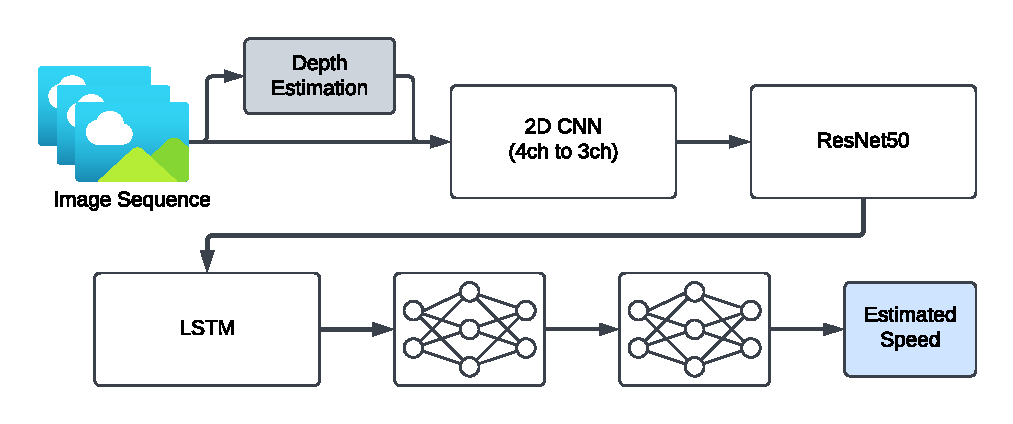
\includegraphics[width=\linewidth,keepaspectratio]{img/vo_arch.pdf}
\caption{Architecture of the visual odometry model. A convolutional
neural network (CNN) was used to reduce input RGB-D images from 4 to 3
channels, then those were run through a pre-trained ResNet and fed into
an LSTM module to detect temporal relationships. Two fully-connected
linear layers were used to reduce the LSTM output to a single estimated
speed (blue).}\label{fig:vo_arch}
\end{figure}

Data was input to the model as sequences of 59 images, each sequence
corresponding to one minute of mowing operations in real time. For each
epoch, 923 sequences were used for training and 113 were used for
testing. Training was performed for 50 epochs, with loss given by the
mean square error (MSE) between the predicted speed and the ground-truth
speed found from associated telematics data. The MSE was chosen for the
loss function because it is appropriate for use with quantitative
regression problems such as this one, and it more heavily penalizes
larger errors, encouraging the model to converge to near the optimal
values more quickly. The ADAM optimizer was used to adjust model weights
according to those calculated losses, as it is a commonly accepted
optimizer in many computer vision tasks that is still advanced and
effective for experimental training
\parencite{Reddi_ConvergenceAdam_2018}.

An additional dataset, with a much higher sample rate (30 Hz) and a
well-characterized speed distribution---collected by recording from the
dashboard of an automobile traveling along a roadside at constant
speed---was also used to train this model. That more tightly controlled
dataset was used for validation, to confirm if the model could be
trained for robustness across related domains, and to help understand
the effect of sample rate on neural network VO. This additional dataset
was split into 336 image sequences for training and 145 for testing. In
order to encourage further development and project transparency, all
code developed for this project is open-source and available online
\parencite{Wiegman_MsThesisRepo_2025}.

\clearpage


\chapter{RESULTS \& DISCUSSION}\label{results-discussion}

\section{Data Collection System Reliability}\label{sec:uptime}

\subsection{First Season (2023)}\label{sec:uptime_2023}

Monitoring of mowing operations suffered from poor uptime throughout the
first year's deployment. An overview of the uptime for telematics,
cameras, and both simultaneously is shown in
Figure~\ref{fig:uptime_2023}, derived from the GPS data recorded by both
systems.

\begin{figure}[h]
\centering
\includegraphics[width=\linewidth,height=2.5in,keepaspectratio]{img/uptime_2023.png}
\caption{Timeline showing when different parts of the data collection
system were properly recording during the 2023 mowing season. There were
significant gaps in coverage both on individual tractors and across the
effort for the season as a whole.}\label{fig:uptime_2023}
\end{figure}

As mentioned in the figure caption, the data collection system missed
significant gaps throughout the season. The telematics loggers were the
most reliable part of the system, as their only weakness was the
occasional drop in GPS signal; otherwise they were almost always online
and logging. There were only two noticeable gaps in the telematics
coverage. The first is on Tractor02 in late August (where the cameras
were working for a time without it), and this was not a failure of the
recording system; that set of logs from the telematics systems was
corrupted and lost after those monitored operations were successfully
recorded. The second gap, on Tractor03 around the same period, is more
mysterious.

A flaw in the system was the inability for cameras to receive GPS signal
reliably before beginning to record, which caused some recordings to
save incorrect timestamps (off by multiple years, in some cases) or no
GPS data at all---which would mean it could not be reliably
time-synchronized with any other data. This was corrected mid-season by
adding a GPS speed trigger to the program in Configuration \#3 (see
Figure~\ref{fig:config3}), which required the GPS to obtain a signal and
report the mower moving before the camera would begin recording. This
added some latency to the startup, but greatly improved the quality of
data recorded by the system, so it was considered a worthwhile
trade-off.

The largest flaw in the system was the frequent failure of the camera
systems to persist after more than a few days from installation or
maintenance. The firmware configurations used at the time
(Configurations \#1-3) all relied on a software-based power-trigger that
started with the tractor's keyed power, as explained in
Section~\ref{sec:methods_camera}. The weakness of this configuration was
that it is incompatible with automatic rebooting after power failure. As
a result, whenever cameras ran completely out of battery between mowing
sessions (verified in more detail in Section~\ref{sec:manual_results})
they would not automatically reboot into the same configuration upon
being recharged by the tractor's power system. This resulted in the
cameras functioning as expected for up to a few days, before running out
of battery and not recording again until reset during maintenance. This
is visible in Figure~\ref{fig:uptime_2023} as the tendency for the
cameras (grey) to be present only for a short period after maintenance
dates (red lines).

Another simple measure of uptime is the geographical coverage of the
system throughout the season. Figure~\ref{fig:counties23} shows all
counties in which GPS-synchronized data was recorded in 2023 on both
camera and telematics simultaneously, as well as all counties in which
partial, non-synchronized GPS data was recorded.

\begin{figure}[h]
\centering
\includegraphics[width=\linewidth,height=3in,keepaspectratio]{img/counties_2023.png}
\caption{Counties in which fully monitored mowing operations took place
during 2023. Gold counties indicate GPS-synchronized data from camera
and telematics simultaneously, while grey counties indicate
non-synchronized data from camera or telematics, not
simultaneously.}\label{fig:counties23}
\end{figure}

\subsection{Second Season (2024)}\label{second-season-2024}

The system was far more reliable in the second season, as many of the
teething issues were characterized and solved during the off-season. An
overview of the uptime for telematics, cameras, and both simultaneously
is shown in Figure~\ref{fig:uptime_2024}, derived from the GPS data
recorded by both systems.

\begin{figure}[h]
\centering
\includegraphics[width=\linewidth,height=2.5in,keepaspectratio]{img/uptime_2024.png}
\caption{Timeline showing when different parts of the data collection
system were properly recording during the 2024 mowing season. There is
significantly more and better coverage than the previous year's timeline
shown in Figure~\ref{fig:uptime_2023}.}\label{fig:uptime_2024}
\end{figure}

There are some gaps in this coverage, albeit less than in 2023. In some
cases (for example, Tractor02 in July), cameras did not record even
though the telematics system recorded activity. Some of these were due
to flaws in the human interface to the system; improperly anchored
strain relief on some units meant that the camera's power cable could be
disconnected if the operator opened the window too widely. Once this
issue was identified, a more controlled strain relief mount---and some
tape to reinforce any loose connections---was installed in all systems,
and that particular issue was effectively prevented for the rest of the
season.

Another human interfacing flaw identified during this season was that of
the switched power connection to the tractor's electrical system. Due to
the geometry of the connector and its placement in the cabin, it could
be crushed by the operator's chair if positioned in a certain way. (The
solution chosen for this problem was simply to remove the systems from
tractors with especially tall operators---who needed their seats to be
in the problematic positions---and re-deploy them in tractors with a
more compatible operator.) As with the window problem, the chosen
solution was able to prevent this issue from happening to the same
system again. However, it must be acknowledged that this was only a
stopgap solution. A more universal answer would be to use a specialized
right-angle or low-profile connector that leaves proper clearance for
the operator's seat.

Another simple measure of uptime is the geographical coverage of the
system throughout the season. Figure~\ref{fig:counties24} shows all
counties in which GPS-synchronized data was recorded in 2024 on both
camera and telematics simultaneously, as well as all counties in which
partial, non-synchronized GPS data was recorded.

\begin{figure}[h]
\centering
\includegraphics[width=\linewidth,height=3in,keepaspectratio]{img/counties_2024.png}
\caption{Counties in which monitored mowing operations took place during
2024. Gold counties indicate GPS-synchronized data from camera and
telematics simultaneously, while grey counties indicate non-synchronized
data from camera or telematics, not
simultaneously.}\label{fig:counties24}
\end{figure}

The conditions experienced throughout the mowing season are quite harsh
on the equipment, explaining some of the failure rates observed in the
results above. One hazard that is rarer but consistent (observed in both
years) was that of debris launched up by the towed mower and back at the
cabin. If given enough speed, even a small object can impart enough
energy to shatter the window glass on which the camera is mounted, as is
seen in Figure~\ref{fig:shatter}.

\begin{figure}[h]
\centering
\includegraphics[width=5in,height=\textheight,keepaspectratio]{img/shatter.png}
\caption{\emph{Left:} View of an implement-facing camera, facing typical
dusty, hot, sun-exposed operating conditions. \emph{Right:} View from
the same camera, one second later, after the tractor's windshield
shattered upon impact with a piece of mower-launched
debris.}\label{fig:shatter}
\end{figure}

\clearpage
\subsection{Year-to-Year Trends}\label{sec:conclude_yty}
A chart showing the difference in recording uptimes is shown in
Figure~\ref{fig:uptime_hours}, proving that the improved data collection
protocols established for 2024 were an improvement on all fronts. The
increased reliability was primarily due to a significantly improved
camera configuration (improved uptime by an order of magnitude!). The
process of developing that optimized procedure is given in
Section~\ref{sec:methods_camera}. Otherwise, improvements in uptime from
2023 to 2024 came from a more aggressive maintenance schedule; as should
be clear from the difference between Figure~\ref{fig:uptime_2023} and
Figure~\ref{fig:uptime_2024}, researchers went into the field to collect
data significantly more often in the second season than in the first.
This enabled more frequent error correction and more opportunities to
notice potential problems sooner.

\begin{figure}[h]
\centering
\includegraphics[width=5in,height=\textheight,keepaspectratio]{img/uptime_hours.png}
\caption{Number of unique hours recorded by each piece of equipment and
simultaneously recorded by both. Camera reliability increased even more
than telematics, though both improved
year-on-year.}\label{fig:uptime_hours}
\end{figure}

\section{On-Road Operations}\label{sec:road_time}

A significant risk factor for roadside workers is their proximity to
traffic. Being close to fast-moving vehicles is dangerous, and being on
the actual lanes for traffic (Zone 1) is even more so. To study the
frequency with which professional tractor operators take on these risks,
another measurement was taken of the proportion of mowing time spent
with the mower extending onto the road surface, including the shoulder
if not the actual road lanes. These measurements for 2023 and 2024,
respectively, are shown in Figure~\ref{fig:shoulder23} and
Figure~\ref{fig:shoulder24}, segregated by road type in both cases.

\begin{figure}[h]
\centering
\includegraphics[width=\linewidth,height=2.5in,keepaspectratio]{img/shoulder_2023.png}
\caption{Operators were much more likely to drive on-road on rural
roads.}\label{fig:shoulder23}
\end{figure}

\begin{figure}[h]
\centering
\includegraphics[width=\linewidth,height=2.5in,keepaspectratio]{img/shoulder_2024.png}
\caption{Operators spent a significant portion of their time driving at
least partially on the shoulder, if not on the road
lanes.}\label{fig:shoulder24}
\end{figure}

These show that tractor operators were much more likely to tow their
mower on-road or at least on-shoulder on rural roads. A significant
reason for this is the very narrow shoulder on many of those roads;
there often is not enough space for the mower to physically fit entirely
off-road. While the practice is still risky compared to staying off the
road entirely, it should also be acknowledged that it is less risky on
rural roads, where traffic is usually lower-speed and less frequent,
than it would be on divided highways.

These results may inspire a change in operating procedures to encourage
safer practices, or spur the development of new roadside vegetation
control technologies that do not require such wide equipment that it
cannot fit on narrow rural shoulders.

\section{Validation Process}\label{sec:results_val}

\subsection{Manual GPS Testing}\label{sec:manual_results}

Initial tests of basic mounting hardware and firmware programming
performed on university-owned tractors led to two useful results. The
first was that suction cup mounts were not reliable enough in the dusty,
high-vibration environment of a working tractor, as all the units
installed tended to fall down within hours or days of initial
deployment. Adhesive-based mounts proved to be a much more robust option
instead. Secondly, reconfiguring the camera firmware in the field proved
to be fast and convenient enough to do onsite without disrupting the
operators for any significant time, so cameras could simply have their
memory card exchanged, their configuration updated, and redeployed on
the spot: no need for changing out the entire camera unit.

A shortcoming of the GoPro platform chosen for this study is that it
cannot charge its own battery while recording
\parencite{GoProSupport_HowChargeCamera_2023}. As a result, the battery
will slowly drain even if the camera is connected to power. This was
verified by connecting the camera through a USB power meter and
measuring the average power draw in various situations. With no battery
installed, the camera draws the same amount of power from the charger as
it does with a partially-charged battery installed, suggesting that no
additional power is drawn for charging the battery.

In initial firmware configurations, two major flaws were the inability
to retain configuration after power loss and the lack of reliable GPS
metadata, as mentioned in Section~\ref{sec:uptime_2023}. Manual tests
were the primary method of iteration when discovering these problems and
attempting to solve them.

After discovering that GPS metadata was unreliable, GPS speed trigger
was added to the configuration (see Figure~\ref{fig:config3}), which
required the camera to obtain a GPS signal and report movement before it
would begin recording. The GPS trigger was tested on foot, bicycle, and
automobile to ensure that it functioned reliably at low, medium, and
high speeds, and all GPS-triggered recordings successfully acquired a
quality GPS signal before starting to record.

To solve the configuration-loss on power-loss issue, a more significant
system architecture change was found necessary. There exists an option
in the firmware to automatically reboot into a given configuration upon
restoring power (\texttt{WAKE=2}), but this is incompatible with
triggering the camera with keyed power. Keyed power, upon being switched
on, changes the camera's input voltage from 0 to 5V in a single step.
This provides one ``rising edge'' in the USB signal. If the camera is
configured with \texttt{WAKE=2}, then that rising edge causes the camera
to boot up from a powered off state. However, if the camera was
configured to wait for USB power before \emph{recording}, it would never
record, because the voltage is already at the maximum of 5V and cannot
``rise'' to provide another rising edge signal. At the time that this
flaw was discovered, the GPS speed trigger had already been in use, so
it was decided to remove the power trigger entirely, and relying on the
combination of the WAKE trigger and the GPS speed trigger.

To ensure that the camera started from the same WAKE state with each
instance of keyed power, the battery was removed entirely: the cameras
were run purely on keyed power. However, this meant that the cameras
could not run any dynamic processes between powered-on periods,
including the real-time clock (RTC) and periodically connecting to GPS.
Having a regular connection to GPS aids the camera in quickly locking
onto a full GPS signal when powered up; lacking this, it may take some
time for the GPS to connect after powering on. While that problem was
found insurmountable, the RTC problem was solved by adding a GPS time
synchronization parameter to the firmware configuration
(\texttt{MSYNC=1}), which resets the RTC on each boot-up with the time
received from GPS. (While this feature is not officially listed as
supported on the Hero 8 cameras used in this study, the configuration
worked correctly in manual and automated testing, recording accurate
timing metadata.)

\subsection{Automated Reliability
Testing}\label{sec:test_rig_results}

The automated testing system was used to gather quantitative results
about the camera triggering reliability and latency. A timeline of
programmed movements and the corresponding recordings is shown in
Figure~\ref{fig:rig_results}.

\begin{figure}[htb]
\centering
\includegraphics[width=5.5in,height=\textheight,keepaspectratio]{img/testrig_results.png}
\caption{The automatic camera properly triggered recording for 80\% of
movements, capturing 64\% of total time spent in motion with an average
latency of 109 seconds or 1.81 minutes.}\label{fig:rig_results}
\end{figure}


\begin{figure}[htb]
\centering
\includegraphics[height=2.5in,keepaspectratio]{img/testrig_results_cov.png}
\caption{Most motions were automatically captured with high coverage,
but sometimes the camera started recording late or did not start at
all.}\label{fig:rig_capture}
\end{figure}

\begin{figure}[htb]
\centering
\includegraphics[height=2.5in,keepaspectratio]{img/testrig_results_lat.png}
\caption{Of recordings that successfully triggered, almost all of them
started recording within two minutes of the machine starting to
move.}\label{fig:rig_latency}
\end{figure}

After the many issues with power failures and GPS metadata in the 2023
mowing season, the automated test system was conceived as a way to
automatically run camera firmware configurations through a lengthy
battery of tests. The repeated power cycles and simple movements test
the reliability of the new firmware; initial tests had difficulty
triggering the camera at the correct times or after multiple power
cycles, but the final firmware developed in this study was quite
successful on the system, as stated in the Figure~\ref{fig:rig_results}
caption.

The movements in which the camera was late to record, or failed to
record at all, were due to the camera failing to obtain a GPS signal and
positively detect its movement. However, as shown in the movements which
started recording late, the camera configuration was still flexible
enough to start recording as soon as a good enough signal could be
obtained, even if it was not directly correlated with the keyed power
input. This adds some robustness to the system for long-term deployments
in places that may have intermittent GPS signal, such as along roads
with tunnels, steep cliffs, or heavy foliage overhead. The distribution
of motion coverage is shown in Figure~\ref{fig:rig_capture}, proving
that the system tends to capture the full duration of events for which a
strong movement signal is measured. The distribution of startup latency
in recordings is shown in Figure~\ref{fig:rig_latency}, which suggests
that the system was quite reliable at beginning to record promptly after
movement starts; long periods of undetected and unrecorded movements are
rare.

\clearpage
\section{Obstacle Encounters}\label{sec:obstacles}
\subsection{First Season (2023)}\label{first-season-2023}
Although limited data was collected in 2023, there was still enough to
measure a significant number of encounters with many kinds of obstacles.
The number of encounters with up to ten kinds of obstacles are shown in
Figure~\ref{fig:obs23r} and Figure~\ref{fig:obs23h} for rural roads or
highways, respectively.

Posts (a catch-all category for any narrow vertical obstacles that were
not road signs) and signs were the most common obstacles by far, with
more posts in highway environments and more signs along rural roads.
Mailboxes were quite common along rural roads but absent on highways.

In all cases, operators were generally successful in maneuvering around
obstacles without touching them. In the situations where the mower made
contact with an obstacle, most of the time the obstacle was left without
any permanent damage (only ``touched''). However, a small but
quantifiable number of situations ended with the mower permanently
damaging the obstacle (the darkest bars in Figure~\ref{fig:obs23r} and
Figure~\ref{fig:obs23h}). While these are regrettable, this provides an
effective baseline level of performance for normal human operators
performing conventional roadside vegetation control.

This data could be useful for comparing against other vegetation control
systems, including autonomous mowing robots, as a benchmark that should
be met or exceeded before implementation. Additionally, this data shows
which classes of obstacles are more common than others; new systems
could prioritize development towards handling the most common kinds of
obstacles first.

\subsection{Second Season (2024)}\label{second-season-2024-1}

The number of encounters with up to ten kinds of obstacles are shown in
Figure~\ref{fig:obs24r} and Figure~\ref{fig:obs24h} for rural roads or
highways, respectively. While the distribution of obstacles did not
change to any incredible degree, note that these plots consider obstacle
encounters from a significantly larger dataset (more hours of
operations) than the previous year's.

\begin{figure}[ph]
\centering
\includegraphics[width=6in,height=\textheight,keepaspectratio]{img/obstacles_2023r.png}
\caption{A plot of the obstacles encountered during 2023 mowing
operations on rural roads. (From 68.5 hours of monitored
operations.)}\label{fig:obs23r}
\end{figure}

\begin{figure}[ph]
\centering
\includegraphics[width=6in,height=\textheight,keepaspectratio]{img/obstacles_2023h.png}
\caption{A plot of the obstacles encountered during 2023 mowing
operations on highway roads. (From 41.8 hours of monitored
operations.)}\label{fig:obs23h}
\end{figure}

\begin{figure}[ph]
\centering
\includegraphics[width=6in,height=\textheight,keepaspectratio]{img/obstacles_2024r.png}
\caption{A plot of the obstacles encountered during 2024 mowing
operations on rural roads. (From 311 hours of monitored
operations.)}\label{fig:obs24r}
\end{figure}

\begin{figure}[ph]
\centering
\includegraphics[width=6in,height=\textheight,keepaspectratio]{img/obstacles_2024h.png}
\caption{A plot of the obstacles encountered during 2024 mowing
operations on highway roads. (From 374 hours of monitored
operations.)}\label{fig:obs24h}
\end{figure}

\clearpage
\section{Visual Odometry}\label{sec:results_vo}
After 50 epochs of training on real timelapse image sequences recorded
in the 2024 season, the model was able to converge on a rough
approximation of the correct values, as shown in
Figure~\ref{fig:vo_timelapse}. The model's predictions gave mixed
results, with significant noise and error in some cases, though the
overall distribution of predictions resembles that of the ground truth
values. However, estimated values were noisy and unpredictable, only
weakly predictive of the true speed. An interesting feature of the model
lies in the ``floor'' observable in the predicted outputs. Since the
predicted speed never strayed below about 2 m/s, it seems that a strong
bias was learned in the fully-connected layers near the end of the
model.

\begin{figure}[h]
\centering
\includegraphics[width=\linewidth,height=3in,keepaspectratio]{img/vo_timelapse.png}
\caption{Results of training on timelapse
dataset.}\label{fig:vo_timelapse}
\end{figure}

This performance is quite poor compared to state-of-the-art results
found in the literature. Purely monocular VO is a challenging computer
vision task, less commonly done effectively compared to methods that use
stereo cameras, panoptic imaging, LIDAR, or other sensor augmentations.
However, some success \emph{has} been reported in the literature before
\parencite{HerreraGranda_MonocularVisualSlam_2024}, so this should not be
an impossible task. The model was later trained on the validation data
set, as explained in Section~\ref{sec:methods_vo}, for 10 epochs, and
the results are shown in Figure~\ref{fig:vo_val}.

\begin{figure}[h]
\centering
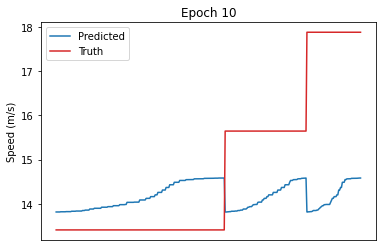
\includegraphics[width=\linewidth,height=3in,keepaspectratio]{img/automobile-training.png}
\caption{Results of training on validation (control)
dataset.}\label{fig:vo_val}
\end{figure}

This process also shows quite poor performance, similar or worse to that
of Figure~\ref{fig:vo_timelapse}. As this was trained on normal,
high-framerate sequences, this suggests that the problem does not
necessarily lie in any specific intractability inherent to timelapse
data. Several possible sources of error seem likely upon further
reflection, but testing further would require more time and resources
than are available at present. A lack of complexity in the model
architecture itself may have been a large source of error for this
process; the architecture summarized in Figure~\ref{fig:vo_arch} was
deliberately simplified and condensed compared to that of the most
performant models in the literature in order to reduce its computational
and memory requirements. A more sophisticated model architecture may
allow a more effective model to be trained for this subject. Another,
more specific potential problem with the tested model lies in the LSTM
layer; relatively small LSTM layers were used, including only 8 cells,
each with 4 hidden nodes. Particularly if combined with a lack of
requisite complexity earlier in the stack, it may have been unrealistic
to expect the model to effectively extract the correct information into
only that space. While LSTM layers tend to run slowly and require
relatively heavy computational loads, those used in this model were
unidirectional and therefore should scale up to moderate sizes without
excessive load. Alternatively, a simpler kind of temporally-dependent
layer could be used in place of the LSTM, such as a Gated Recurrent Unit
(GRU) or Temporal Convolutional Network (TCN), which require less
computational resources than LSTM layers do.

\chapter{CONCLUSION}\label{conclusion}

\section{In-Field Data Collection Processes}\label{sec:conclude_data}

The roadside mowing environment is a very challenging one in which to
collect data. Monitoring equipment must be able to withstand harsh
swings in temperature, direct sunlight, high risk of moisture and dust
ingress, heavy vibration, and even high-velocity debris collision, as
shown in Figure~\ref{fig:shatter}. For these reasons, action-sports
cameras are recommended when photographs or video recordings are
desired. The GoPro cameras used in this study were impeccably robust in
terms of physical resilience (at least twice they outlived the windows
to which they were attached!). Additionally, the Labs firmware
\parencite{Newman_GoproLabs_2024} enabled a very flexible system for
programming deterministic behavior, allowing advanced configurations for
adaptability to a wide array of image collection tasks. For logging
telematics, most standard agricultural units should be effective. The
roadside is not significantly harsher in terms of environmental
conditions than the farm field, so equipment that is designed for
general agricultural use should be equally effective for use in roadside
mowing.

The fundamental nature of roadside work means that all but the most
short-term of experiments must be sent on long journeys, often through
remote locations and sometimes across rugged terrain. This adds risks to
the data collection process; when the system encounters some kind of
fault, there are not necessarily guarantees of prompt service. To manage
this condition, it is recommended to configure systems to automatically
recover from faults whenever possible. However, such a simple solution
is hardly foolproof or holistic in and of itself. Another way to control
for the potential of interruptions in data collection is to schedule
regular check-ins. As noted in Section~\ref{sec:conclude_yty} above,
part of the reason that the system from this project improved in
reliability in the 2024 season was the fact that the maintenance
schedule included significantly more frequent hands-on interactions with
the monitoring equipment. Any time that the systems failed for some
reason, having a prompt check-in to notice and remedy the problem
reduced total system downtime, preventing any gaps in data collection
from growing too severe.

\section{Evidence-Based Mowing Standards}\label{sec:conclude_mow}

The primary metrics for mower performance that came from this study
revolve around the rate of encounters with obstacles and the proportion
of mowing time spent in the Zone 1 (paved road surface). The most
accurate estimate of human operators' obstacle encounter rates on
Indiana roads is likely to be Figure~\ref{fig:obs24h} and
Figure~\ref{fig:obs24r}, as they are based on analysis of significantly
more operating hours than the first season's results provided. These two
plots show that human mower operators make contact with obstacles as
frequently as 8 times per hour, and they cause permanent damage to
obstacles at rates of up to 0.4 times per hour. Likewise,
Figure~\ref{fig:shoulder23} and Figure~\ref{fig:shoulder24} show that
human operators spend as little as 10\% of their time fully off-road on
rural routes, and as little as 40\% of their time fully off-road on
divided highway routes. Therefore, future roadside vegetation management
technologies need only meet those basic standards in order to have
quantitatively equivalent performance to human-operated mowers. It is
likely that future technologies---such as autonomous roadside
mowers---could even perform significantly better than those minimum
standards, which would lead to greater safety for the public and reduced
outlay on property damage: major improvements to the process of roadside
vegetation control as a whole.

\chapter{FUTURE WORK}\label{future-work}

The results of the analysis of collected data, as shown particularly in
Section~\ref{sec:obstacles}, provide a much clearer understanding of the
typical challenges faced by mower operators in Indiana, in addition to
proving the robustness of the data collection methods outlined in this
document. Simulations of the roadway environment, such as
\textcite{Mardikes_ConstructingDigitalTwin_2025}, could use these
obstacle encounter rates to more accurately model the rate at which
different obstacles are likely to appear. Additionally, this information
has been provided to INDOT, and they may be able to use it to better
prioritize their safety communications and make other policy decisions
based on a more accurate and up-to-date understanding of the real-world
roadside mowing environment and associated typical mower operator
behavior. Finally, the novel research problem of effectively estimating
visual odometry from timelapse data remains unsolved, though a
refinement of the methods attempted here with a more sophisticated
architecture and/or additional computational resources may be a
relatively simple path to acceptable performance.


% CHAPTER TEXT GOES HERE ^^^^^


\makeatletter  % commented out on 2022-01-26
  \defbibenvironment{bibliography}
    {%
      \list
        {%
          \printtext[labelnumberwidth]%
          {%
            \printfield{prefixnumber}%
            \printfield{labelnumber}%
          }%
        }%
        {%
          \setlength{\bibhang}{1in} %%%%% was 0pt
          \setlength{\itemindent}{1in}%  -\leftmargin} %%%%% was 0pt
          \setlength{\itemsep}{\bibitemsep}%
          \setlength{\leftmargin}{0pt}%  .22in} % 0.42in}
          \setlength{\parsep}{\bibparsep}%
          \setlength{\rightmargin}{0.33in}%
        }%
    }
    {\endlist}
    {\item}
\makeatother  % commented out on 2022-01-26

% \immediate\setlength{\labelnumberwidth}{1.5in} %%%%% was commented out
\setlength{\labelwidth}{1.5in}

{%
  % Make _ in URLs visible.
  % \def\t{\char'137}%
  \catcode`*=\active
  \def*{\char'137}%  \char'137 is _
  \PrintBibliography
}

% Appendices are optional.  Not all theses contain appendices.
% An appendix is used for supplementary illustrative material,
% original data, computer programs, and other material that is not
% necessarily appropriate for inclusion within the text of your
% thesis.
% Reference: TM2017 page 33.
%
% Use ``\appendix'' for one appendix or ``\appendices'' for more than
% one appendix.
% \appendix


% My filename conventions:
%     FILE THAT START WITH    ARE
%     ap-                     appendices
%     ch-                     chapters
%     gr-                     graphics
%     pa-                     packages
%     z                       temporary files

  % % "About Appendices" appendix.
  % \include{ap-about-appendices}

  % % Accessibility.
  % \include{ap-accessibility}
  
  % % "Bugs" appendix.
  % \include{ap-bugs}

  % % Check margins.
  % \include{ap-check-margins}

  % % Demonstrate how to do separate appendices per chapter.
  % \include{ap-chapter-appendices}

  % % Citations and references.
  % \include{ap-citations-references}

  % % Common mistakes.
  % \include{ap-common-mistakes}

  % % Defining commands.
  % \include{ap-defining-commands}

  % % Deprecated software.
  % \include{ap-deprecated-software}

  % % Figures.
  % \include{ap-figures}

  % % Frequently Asked Questions.
  % \include{ap-frequently-asked-questions}

  % % Graphics.
  % \include{ap-graphics}

  % % How to debug LaTeX Problems.
  % \include{ap-how-to-debug-latex-problems}

  % % Ignore these references.
  % \include{ap-ignore-these-references}

  % % Logos.
  % \include{ap-logos}

  % % Numbers and Units.
  % \include{ap-numbers-and-units}

  % % Resources.
  % \include{ap-resources}

  % % Tables.
  % \include{ap-tables}

  % % Special characters.
  % \include{ap-special-characters}

  % % Testing.
  % \include{ap-testing}

  % % Text.
  % \include{ap-text}

  % % Video.
  % % \include{ap-video}

  % % Astronomy.
  % \include{ap-astronomy}

  % % Biology.
  % \include{ap-biology}

  % % Chemistry.
  % \include{ap-chemistry}

  % % Computer Science.
  % \include{ap-computer-science}

  % % Electrical Engineering.
  % \include{ap-electrical-engineering}

  % % Linguistics.
  % \include{ap-linguistics}

  % % Mathematics.
  % \include{ap-mathematics}

  % % Music.
  % \include{ap-music}

  % % Physics.
  % \include{ap-physics}

  % Notes and footnotes are optional.
  % Reference: TM2017 page 34.
  % I have not implemented this yet.  Mark Senn 2002-06-03

  % A vita is optional for masters theses
  % and required for doctoral dissertations.
  % Reference: TM2017 page 13.
  % \include{ap-vita}

  % Listing or including publications(s) is optional.
% \include{ap-publications}
% \includepdf[scale=0.9, pages=1]{ztemp-sgopalsa-paper.pdf}
% \includepdf[offset=-1.5truein 0.25truein, scale=0.9, pages=1]{ztemp-sgopalsa-paper.pdf}
% \includepdf[offset=-1.5truein 0.2truein,  scale=0.9, pages=2]{ztemp-sgopalsa-paper.pdf}
% \includepdf[offset=-1.5truein 0.2truein,  scale=0.9, pages=3]{ztemp-sgopalsa-paper.pdf}
% \includepdf[offset=-1.5truein 0.2truein,  scale=0.9, pages=4]{ztemp-sgopalsa-paper.pdf}
% \includepdf[offset=-1.5truein 0.2truein,  scale=0.9, pages=5]{ztemp-sgopalsa-paper.pdf}
% \includepdf[offset=-1.5truein 0.2truein,  scale=0.9, pages=6]{ztemp-sgopalsa-paper.pdf}
% \includepdf[offset=-1.5truein 0.2truein,  scale=0.9, pages=7]{ztemp-sgopalsa-paper.pdf}

  % Print the index.
  % The index is optional.
  \pdfbookmark{INDEX}{index}
  \printindex

  % If \ZZshowcolophon is true, print the colophon.
  % \pdfbookmark{COLOPHON}{colophon}
  % \ifthen{\equal{true}{\ZZshowcolophon}}
  %   {\include{ap-colophon}}

% LaTeX won't read after the \end{document} command.
% You can put notes to yourself or LaTeX input not
% ready for use after "\end{document}" if you'd like.
\end{document}
